%% 由 build/emit_tex.py 生成（生成物，勿手改）；定制请放 user_style.tex / user_meta.yaml
\chapter{Matplotlib及其基本使用}\label{matplotlibux53caux5176ux57faux672cux4f7fux7528}

\section{01
基本绘图：折线、散点、条形、饼图、直方图、箱线图等}\label{ux57faux672cux7ed8ux56feux6298ux7ebfux6563ux70b9ux6761ux5f62ux997cux56feux76f4ux65b9ux56feux7bb1ux7ebfux56feux7b49}

\begin{quote}
本节对应原版 5.1 的内容，并增补学习目标、常见误区、思考题与延伸阅读。
配套图：\texttt{figures/05-matplotlib/basic\_plots.png}（由
\texttt{build/make\_chap5\_figures.py} 生成）。
\end{quote}

\subsection{本节目标}\label{ux672cux8282ux76eeux6807-13}

\begin{itemize}
\tightlist
\item
  会用 \texttt{matplotlib.pyplot} 绘制 6 种最常用的基础图表；
\item
  理解面向对象接口（\texttt{fig} /
  \texttt{ax}）与``函数式''接口（\texttt{plt.plot}）的关系；
\item
  会为图表添加标题、坐标轴标签、图例；
\item
  接触热力图、误差棒图、极坐标、3D、等高线等扩展图型。
\end{itemize}

\subsection{先修}\label{ux5148ux4fee-13}

\begin{itemize}
\tightlist
\item
  Python 基础语法；NumPy
  数组（\texttt{np.linspace}、\texttt{np.arange}、随机数）。
\end{itemize}

\subsection{官方文档/参考入口}\label{ux5b98ux65b9ux6587ux6863ux53c2ux8003ux5165ux53e3-2}

\begin{itemize}
\tightlist
\item
  Matplotlib
  官方快速开始：https://matplotlib.org/stable/tutorials/introductory/quick\_start.html
\item
  Matplotlib 图型画廊：https://matplotlib.org/stable/gallery/index.html
\end{itemize}

\begin{center}\rule{0.5\linewidth}{0.5pt}\end{center}

\subsection{\texorpdfstring{1.1
快速开始：\texttt{import\ matplotlib.pyplot\ as\ plt}}{1.1 快速开始：import matplotlib.pyplot as plt}}\label{ux5febux901fux5f00ux59cbimport-matplotlib.pyplot-as-plt}

\begin{quote}
Matplotlib
有两种风格：\textbf{函数式}（\texttt{plt.plot}，自动管理当前图）与\textbf{面向对象}（\texttt{fig,\ ax\ =\ plt.subplots()}，手动管理
Axes）。本教材优先介绍函数式，第 2 节再切换到面向对象。
\end{quote}

\begin{Shaded}
\begin{Highlighting}[]
\ImportTok{import}\NormalTok{ matplotlib.pyplot }\ImportTok{as}\NormalTok{ plt}

\NormalTok{x }\OperatorTok{=}\NormalTok{ [}\DecValTok{1}\NormalTok{, }\DecValTok{2}\NormalTok{, }\DecValTok{3}\NormalTok{, }\DecValTok{4}\NormalTok{, }\DecValTok{5}\NormalTok{]}
\NormalTok{y }\OperatorTok{=}\NormalTok{ [}\DecValTok{1}\NormalTok{, }\DecValTok{4}\NormalTok{, }\DecValTok{9}\NormalTok{, }\DecValTok{16}\NormalTok{, }\DecValTok{25}\NormalTok{]}

\NormalTok{plt.plot(x, y)}
\NormalTok{plt.title(}\StringTok{\textquotesingle{}Simple Plot\textquotesingle{}}\NormalTok{)}
\NormalTok{plt.xlabel(}\StringTok{\textquotesingle{}x axis\textquotesingle{}}\NormalTok{)}
\NormalTok{plt.ylabel(}\StringTok{\textquotesingle{}y axis\textquotesingle{}}\NormalTok{)}
\NormalTok{plt.show()}
\end{Highlighting}
\end{Shaded}

运行后得到一条折线。若在 Jupyter 中，\texttt{plt.show()}
会把图形显示在输出区；在脚本中则弹出窗口（无窗口环境请用
\texttt{plt.savefig}）。

\subsection{1.2
常见基础图表}\label{ux5e38ux89c1ux57faux7840ux56feux8868}

\subsubsection{\texorpdfstring{1.2.1
折线图（\texttt{plot}）}{1.2.1 折线图（plot）}}\label{ux6298ux7ebfux56feplot}

\begin{Shaded}
\begin{Highlighting}[]
\ImportTok{import}\NormalTok{ numpy }\ImportTok{as}\NormalTok{ np}
\ImportTok{import}\NormalTok{ matplotlib.pyplot }\ImportTok{as}\NormalTok{ plt}

\NormalTok{x }\OperatorTok{=}\NormalTok{ [}\DecValTok{1}\NormalTok{, }\DecValTok{2}\NormalTok{, }\DecValTok{3}\NormalTok{, }\DecValTok{4}\NormalTok{, }\DecValTok{5}\NormalTok{]}
\NormalTok{y }\OperatorTok{=}\NormalTok{ [}\DecValTok{1}\NormalTok{, }\DecValTok{4}\NormalTok{, }\DecValTok{9}\NormalTok{, }\DecValTok{16}\NormalTok{, }\DecValTok{25}\NormalTok{]}
\NormalTok{plt.plot(x, y)}
\NormalTok{plt.title(}\StringTok{\textquotesingle{}Simple Plot\textquotesingle{}}\NormalTok{)}
\NormalTok{plt.xlabel(}\StringTok{\textquotesingle{}x axis\textquotesingle{}}\NormalTok{)}
\NormalTok{plt.ylabel(}\StringTok{\textquotesingle{}y axis\textquotesingle{}}\NormalTok{)}
\BuiltInTok{print}\NormalTok{(}\StringTok{\textquotesingle{}x:\textquotesingle{}}\NormalTok{, x)}
\BuiltInTok{print}\NormalTok{(}\StringTok{\textquotesingle{}y:\textquotesingle{}}\NormalTok{, y)}
\end{Highlighting}
\end{Shaded}

\begin{Shaded}
\begin{Highlighting}[]
\NormalTok{x: [1, 2, 3, 4, 5]}
\NormalTok{y: [1, 4, 9, 16, 25]}
\end{Highlighting}
\end{Shaded}

\subsubsection{\texorpdfstring{1.2.2
散点图（\texttt{scatter}）}{1.2.2 散点图（scatter）}}\label{ux6563ux70b9ux56fescatter}

\begin{Shaded}
\begin{Highlighting}[]
\ImportTok{import}\NormalTok{ numpy }\ImportTok{as}\NormalTok{ np}
\ImportTok{import}\NormalTok{ matplotlib.pyplot }\ImportTok{as}\NormalTok{ plt}

\NormalTok{rng }\OperatorTok{=}\NormalTok{ np.random.default\_rng(}\DecValTok{0}\NormalTok{)}
\NormalTok{x }\OperatorTok{=}\NormalTok{ rng.normal(}\DecValTok{0}\NormalTok{, }\DecValTok{1}\NormalTok{, }\DecValTok{60}\NormalTok{)}
\NormalTok{y }\OperatorTok{=} \FloatTok{0.6} \OperatorTok{*}\NormalTok{ x }\OperatorTok{+}\NormalTok{ rng.normal(}\DecValTok{0}\NormalTok{, }\FloatTok{0.4}\NormalTok{, }\DecValTok{60}\NormalTok{)}
\NormalTok{plt.scatter(x, y, s}\OperatorTok{=}\DecValTok{28}\NormalTok{, c}\OperatorTok{=}\StringTok{\textquotesingle{}\#e07b39\textquotesingle{}}\NormalTok{, alpha}\OperatorTok{=}\FloatTok{0.8}\NormalTok{)}
\NormalTok{plt.title(}\StringTok{\textquotesingle{}Scatter Plot\textquotesingle{}}\NormalTok{)}
\BuiltInTok{print}\NormalTok{(}\StringTok{\textquotesingle{}x min/max:\textquotesingle{}}\NormalTok{, }\BuiltInTok{round}\NormalTok{(x.}\BuiltInTok{min}\NormalTok{(), }\DecValTok{3}\NormalTok{), }\BuiltInTok{round}\NormalTok{(x.}\BuiltInTok{max}\NormalTok{(), }\DecValTok{3}\NormalTok{))}
\BuiltInTok{print}\NormalTok{(}\StringTok{\textquotesingle{}y mean:\textquotesingle{}}\NormalTok{, }\BuiltInTok{round}\NormalTok{(y.mean(), }\DecValTok{3}\NormalTok{))}
\end{Highlighting}
\end{Shaded}

\begin{Shaded}
\begin{Highlighting}[]
\NormalTok{x min/max: {-}2.325 1.96}
\NormalTok{y mean: 0.08}
\end{Highlighting}
\end{Shaded}

\begin{quote}
\texttt{s} 控制点面积、\texttt{c} 控制颜色、\texttt{alpha}
控制透明度；\texttt{np.random.default\_rng(0)} 保证结果可复现。
\end{quote}

\subsubsection{\texorpdfstring{1.2.3
条形图（\texttt{bar}）}{1.2.3 条形图（bar）}}\label{ux6761ux5f62ux56febar}

\begin{Shaded}
\begin{Highlighting}[]
\ImportTok{import}\NormalTok{ matplotlib.pyplot }\ImportTok{as}\NormalTok{ plt}

\NormalTok{cats }\OperatorTok{=}\NormalTok{ [}\StringTok{\textquotesingle{}A\textquotesingle{}}\NormalTok{, }\StringTok{\textquotesingle{}B\textquotesingle{}}\NormalTok{, }\StringTok{\textquotesingle{}C\textquotesingle{}}\NormalTok{, }\StringTok{\textquotesingle{}D\textquotesingle{}}\NormalTok{]}
\NormalTok{vals }\OperatorTok{=}\NormalTok{ [}\DecValTok{23}\NormalTok{, }\DecValTok{45}\NormalTok{, }\DecValTok{56}\NormalTok{, }\DecValTok{78}\NormalTok{]}
\NormalTok{plt.bar(cats, vals)}
\NormalTok{plt.title(}\StringTok{\textquotesingle{}Bar Chart\textquotesingle{}}\NormalTok{)}
\NormalTok{plt.xlabel(}\StringTok{\textquotesingle{}Categories\textquotesingle{}}\NormalTok{)}
\NormalTok{plt.ylabel(}\StringTok{\textquotesingle{}Values\textquotesingle{}}\NormalTok{)}
\BuiltInTok{print}\NormalTok{(}\StringTok{\textquotesingle{}vals:\textquotesingle{}}\NormalTok{, vals)}
\BuiltInTok{print}\NormalTok{(}\StringTok{\textquotesingle{}total:\textquotesingle{}}\NormalTok{, }\BuiltInTok{sum}\NormalTok{(vals))}
\end{Highlighting}
\end{Shaded}

\begin{Shaded}
\begin{Highlighting}[]
\NormalTok{vals: [23, 45, 56, 78]}
\NormalTok{total: 202}
\end{Highlighting}
\end{Shaded}

\subsubsection{\texorpdfstring{1.2.4
饼图（\texttt{pie}）}{1.2.4 饼图（pie）}}\label{ux997cux56fepie}

\begin{Shaded}
\begin{Highlighting}[]
\ImportTok{import}\NormalTok{ matplotlib.pyplot }\ImportTok{as}\NormalTok{ plt}

\NormalTok{labels }\OperatorTok{=} \StringTok{\textquotesingle{}Frogs\textquotesingle{}}\NormalTok{, }\StringTok{\textquotesingle{}Hogs\textquotesingle{}}\NormalTok{, }\StringTok{\textquotesingle{}Dogs\textquotesingle{}}\NormalTok{, }\StringTok{\textquotesingle{}Logs\textquotesingle{}}
\NormalTok{sizes }\OperatorTok{=}\NormalTok{ [}\DecValTok{15}\NormalTok{, }\DecValTok{30}\NormalTok{, }\DecValTok{45}\NormalTok{, }\DecValTok{10}\NormalTok{]}
\NormalTok{plt.pie(sizes, labels}\OperatorTok{=}\NormalTok{labels, autopct}\OperatorTok{=}\StringTok{\textquotesingle{}}\SpecialCharTok{\%1.1f\%\%}\StringTok{\textquotesingle{}}\NormalTok{, startangle}\OperatorTok{=}\DecValTok{140}\NormalTok{)}
\NormalTok{plt.title(}\StringTok{\textquotesingle{}Pie Chart\textquotesingle{}}\NormalTok{)}
\NormalTok{plt.axis(}\StringTok{\textquotesingle{}equal\textquotesingle{}}\NormalTok{)}
\BuiltInTok{print}\NormalTok{(}\StringTok{\textquotesingle{}sizes:\textquotesingle{}}\NormalTok{, sizes, }\StringTok{\textquotesingle{}sum:\textquotesingle{}}\NormalTok{, }\BuiltInTok{sum}\NormalTok{(sizes))}
\end{Highlighting}
\end{Shaded}

\begin{Shaded}
\begin{Highlighting}[]
\NormalTok{sizes: [15, 30, 45, 10] sum: 100}
\end{Highlighting}
\end{Shaded}

\begin{quote}
\texttt{autopct} 控制百分比格式，\texttt{startangle}
控制起始角度，\texttt{axis(\textquotesingle{}equal\textquotesingle{})}
保证饼图是正圆。
\end{quote}

\subsubsection{\texorpdfstring{1.2.5
直方图（\texttt{hist}）}{1.2.5 直方图（hist）}}\label{ux76f4ux65b9ux56fehist}

\begin{Shaded}
\begin{Highlighting}[]
\ImportTok{import}\NormalTok{ numpy }\ImportTok{as}\NormalTok{ np}
\ImportTok{import}\NormalTok{ matplotlib.pyplot }\ImportTok{as}\NormalTok{ plt}

\NormalTok{mu, sigma }\OperatorTok{=} \DecValTok{0}\NormalTok{, }\FloatTok{0.1}
\NormalTok{data }\OperatorTok{=}\NormalTok{ np.random.default\_rng(}\DecValTok{5}\NormalTok{).normal(mu, sigma, }\DecValTok{1000}\NormalTok{)}
\NormalTok{counts, bins, patches }\OperatorTok{=}\NormalTok{ plt.hist(data, bins}\OperatorTok{=}\DecValTok{30}\NormalTok{, density}\OperatorTok{=}\VariableTok{True}\NormalTok{)}
\NormalTok{plt.title(}\StringTok{\textquotesingle{}Histogram\textquotesingle{}}\NormalTok{)}
\NormalTok{plt.xlabel(}\StringTok{\textquotesingle{}Value\textquotesingle{}}\NormalTok{)}
\NormalTok{plt.ylabel(}\StringTok{\textquotesingle{}Frequency\textquotesingle{}}\NormalTok{)}
\BuiltInTok{print}\NormalTok{(}\StringTok{\textquotesingle{}bin count:\textquotesingle{}}\NormalTok{, }\BuiltInTok{len}\NormalTok{(patches))}
\BuiltInTok{print}\NormalTok{(}\StringTok{\textquotesingle{}first/last bin:\textquotesingle{}}\NormalTok{, }\BuiltInTok{round}\NormalTok{(bins[}\DecValTok{0}\NormalTok{], }\DecValTok{3}\NormalTok{), }\BuiltInTok{round}\NormalTok{(bins[}\OperatorTok{{-}}\DecValTok{1}\NormalTok{], }\DecValTok{3}\NormalTok{))}
\end{Highlighting}
\end{Shaded}

\begin{Shaded}
\begin{Highlighting}[]
\NormalTok{bin count: 30}
\NormalTok{first/last bin: {-}0.328 0.311}
\end{Highlighting}
\end{Shaded}

\begin{quote}
\texttt{density=True} 时纵轴是概率密度（面积归一为 1）；\texttt{bins}
为分箱数。
\end{quote}

\subsubsection{\texorpdfstring{1.2.6
箱线图（\texttt{boxplot}）}{1.2.6 箱线图（boxplot）}}\label{ux7bb1ux7ebfux56feboxplot}

\begin{Shaded}
\begin{Highlighting}[]
\ImportTok{import}\NormalTok{ numpy }\ImportTok{as}\NormalTok{ np}
\ImportTok{import}\NormalTok{ matplotlib.pyplot }\ImportTok{as}\NormalTok{ plt}

\NormalTok{np.random.seed(}\DecValTok{10}\NormalTok{)}
\NormalTok{data }\OperatorTok{=}\NormalTok{ np.random.normal(}\DecValTok{0}\NormalTok{, }\DecValTok{1}\NormalTok{, }\DecValTok{200}\NormalTok{)}
\NormalTok{data }\OperatorTok{=}\NormalTok{ np.concatenate([data, [}\DecValTok{10}\NormalTok{]])   }\CommentTok{\# 加入一个异常值}
\NormalTok{plt.boxplot(data)}
\NormalTok{plt.title(}\StringTok{\textquotesingle{}Boxplot\textquotesingle{}}\NormalTok{)}
\BuiltInTok{print}\NormalTok{(}\StringTok{\textquotesingle{}outliers \textgreater{} 3:\textquotesingle{}}\NormalTok{, }\BuiltInTok{int}\NormalTok{((data }\OperatorTok{\textgreater{}} \DecValTok{3}\NormalTok{).}\BuiltInTok{sum}\NormalTok{()))}
\BuiltInTok{print}\NormalTok{(}\StringTok{\textquotesingle{}max:\textquotesingle{}}\NormalTok{, }\BuiltInTok{round}\NormalTok{(data.}\BuiltInTok{max}\NormalTok{(), }\DecValTok{2}\NormalTok{))}
\end{Highlighting}
\end{Shaded}

\begin{Shaded}
\begin{Highlighting}[]
\NormalTok{outliers \textgreater{} 3: 1}
\NormalTok{max: 10.0}
\end{Highlighting}
\end{Shaded}

\begin{quote}
箱线图用五数概括（Q1、中位数、Q3、上下须）展示分布，异常值以离群点显示。
\end{quote}

\subsubsection{\texorpdfstring{1.2.7
热力图（\texttt{imshow}）}{1.2.7 热力图（imshow）}}\label{ux70edux529bux56feimshow}

\begin{Shaded}
\begin{Highlighting}[]
\ImportTok{import}\NormalTok{ numpy }\ImportTok{as}\NormalTok{ np}
\ImportTok{import}\NormalTok{ matplotlib.pyplot }\ImportTok{as}\NormalTok{ plt}

\NormalTok{data }\OperatorTok{=}\NormalTok{ np.random.default\_rng(}\DecValTok{7}\NormalTok{).random((}\DecValTok{10}\NormalTok{, }\DecValTok{10}\NormalTok{))}
\NormalTok{plt.imshow(data, cmap}\OperatorTok{=}\StringTok{\textquotesingle{}hot\textquotesingle{}}\NormalTok{, interpolation}\OperatorTok{=}\StringTok{\textquotesingle{}nearest\textquotesingle{}}\NormalTok{)}
\NormalTok{plt.colorbar()}
\NormalTok{plt.title(}\StringTok{\textquotesingle{}Heatmap Example\textquotesingle{}}\NormalTok{)}
\BuiltInTok{print}\NormalTok{(}\StringTok{\textquotesingle{}matrix shape:\textquotesingle{}}\NormalTok{, data.shape)}
\end{Highlighting}
\end{Shaded}

\begin{Shaded}
\begin{Highlighting}[]
\NormalTok{matrix shape: (10, 10)}
\end{Highlighting}
\end{Shaded}

\begin{quote}
\texttt{imshow} 适合展示 2D 数值矩阵；\texttt{cmap}
控制配色，\texttt{colorbar} 加色标。
\end{quote}

\subsubsection{\texorpdfstring{1.2.8
误差棒图（\texttt{errorbar}）}{1.2.8 误差棒图（errorbar）}}\label{ux8befux5deeux68d2ux56feerrorbar}

\begin{Shaded}
\begin{Highlighting}[]
\ImportTok{import}\NormalTok{ numpy }\ImportTok{as}\NormalTok{ np}
\ImportTok{import}\NormalTok{ matplotlib.pyplot }\ImportTok{as}\NormalTok{ plt}

\NormalTok{x }\OperatorTok{=}\NormalTok{ np.arange(}\FloatTok{0.1}\NormalTok{, }\DecValTok{4}\NormalTok{, }\FloatTok{0.5}\NormalTok{)}
\NormalTok{y }\OperatorTok{=}\NormalTok{ np.exp(}\OperatorTok{{-}}\NormalTok{x)}
\NormalTok{yerr }\OperatorTok{=} \FloatTok{0.1} \OperatorTok{+} \FloatTok{0.2} \OperatorTok{*}\NormalTok{ np.sqrt(x)}
\NormalTok{xerr }\OperatorTok{=} \FloatTok{0.1} \OperatorTok{*}\NormalTok{ np.ones\_like(x)}
\NormalTok{plt.errorbar(x, y, xerr}\OperatorTok{=}\NormalTok{xerr, yerr}\OperatorTok{=}\NormalTok{yerr, fmt}\OperatorTok{=}\StringTok{\textquotesingle{}{-}o\textquotesingle{}}\NormalTok{)}
\NormalTok{plt.title(}\StringTok{\textquotesingle{}Errorbar Chart Example\textquotesingle{}}\NormalTok{)}
\BuiltInTok{print}\NormalTok{(}\StringTok{\textquotesingle{}n points:\textquotesingle{}}\NormalTok{, x.size)}
\end{Highlighting}
\end{Shaded}

\begin{Shaded}
\begin{Highlighting}[]
\NormalTok{n points: 8}
\end{Highlighting}
\end{Shaded}

\subsubsection{1.2.9
扩展图型：极坐标、3D、等高线}\label{ux6269ux5c55ux56feux578bux6781ux5750ux68073dux7b49ux9ad8ux7ebf}

\begin{Shaded}
\begin{Highlighting}[]
\ImportTok{import}\NormalTok{ numpy }\ImportTok{as}\NormalTok{ np}
\ImportTok{import}\NormalTok{ matplotlib.pyplot }\ImportTok{as}\NormalTok{ plt}
\ImportTok{from}\NormalTok{ mpl\_toolkits.mplot3d }\ImportTok{import}\NormalTok{ Axes3D}

\CommentTok{\#\# 极坐标}
\NormalTok{r }\OperatorTok{=}\NormalTok{ np.arange(}\DecValTok{0}\NormalTok{, }\DecValTok{2}\NormalTok{, }\FloatTok{0.01}\NormalTok{)}
\NormalTok{theta }\OperatorTok{=} \DecValTok{2} \OperatorTok{*}\NormalTok{ np.pi }\OperatorTok{*}\NormalTok{ r}
\NormalTok{plt.polar(theta, r)}
\NormalTok{plt.title(}\StringTok{\textquotesingle{}Polar Chart\textquotesingle{}}\NormalTok{)}
\BuiltInTok{print}\NormalTok{(}\StringTok{\textquotesingle{}polar points:\textquotesingle{}}\NormalTok{, r.size)}

\CommentTok{\#\# 3D 曲面}
\NormalTok{x }\OperatorTok{=}\NormalTok{ np.linspace(}\OperatorTok{{-}}\DecValTok{5}\NormalTok{, }\DecValTok{5}\NormalTok{, }\DecValTok{100}\NormalTok{)}\OperatorTok{;}\NormalTok{ y }\OperatorTok{=}\NormalTok{ np.linspace(}\OperatorTok{{-}}\DecValTok{5}\NormalTok{, }\DecValTok{5}\NormalTok{, }\DecValTok{100}\NormalTok{)}
\NormalTok{X, Y }\OperatorTok{=}\NormalTok{ np.meshgrid(x, y)}
\NormalTok{Z }\OperatorTok{=}\NormalTok{ np.sin(np.sqrt(X}\OperatorTok{**}\DecValTok{2} \OperatorTok{+}\NormalTok{ Y}\OperatorTok{**}\DecValTok{2}\NormalTok{))}
\NormalTok{fig }\OperatorTok{=}\NormalTok{ plt.figure()}
\NormalTok{ax }\OperatorTok{=}\NormalTok{ fig.add\_subplot(}\DecValTok{111}\NormalTok{, projection}\OperatorTok{=}\StringTok{\textquotesingle{}3d\textquotesingle{}}\NormalTok{)}
\NormalTok{ax.plot\_surface(X, Y, Z, cmap}\OperatorTok{=}\StringTok{\textquotesingle{}viridis\textquotesingle{}}\NormalTok{)}
\BuiltInTok{print}\NormalTok{(}\StringTok{\textquotesingle{}surface shape:\textquotesingle{}}\NormalTok{, Z.shape)}
\NormalTok{plt.close(fig)     }\CommentTok{\# 关闭 3D 图，避免与下面的等高线共用 Figure}

\CommentTok{\#\# 等高线}
\NormalTok{plt.contour(X, Y, Z, colors}\OperatorTok{=}\StringTok{\textquotesingle{}k\textquotesingle{}}\NormalTok{)}
\NormalTok{plt.contourf(X, Y, Z, cmap}\OperatorTok{=}\StringTok{\textquotesingle{}viridis\textquotesingle{}}\NormalTok{)}
\NormalTok{plt.colorbar()}
\BuiltInTok{print}\NormalTok{(}\StringTok{\textquotesingle{}X,Y,Z shapes:\textquotesingle{}}\NormalTok{, X.shape, Y.shape, Z.shape)}
\end{Highlighting}
\end{Shaded}

\begin{Shaded}
\begin{Highlighting}[]
\NormalTok{polar points: 200}
\NormalTok{surface shape: (100, 100)}
\NormalTok{X,Y,Z shapes: (100, 100) (100, 100) (100, 100)}
\end{Highlighting}
\end{Shaded}

\begin{quote}
3D 图需要
\texttt{from\ mpl\_toolkits.mplot3d\ import\ Axes3D}；\texttt{add\_subplot(111,\ projection=\textquotesingle{}3d\textquotesingle{})}
表示 1×1 网格中的第一个子图（详见第 2 节）。
\end{quote}

\begin{figure}
\centering
\pandocbounded{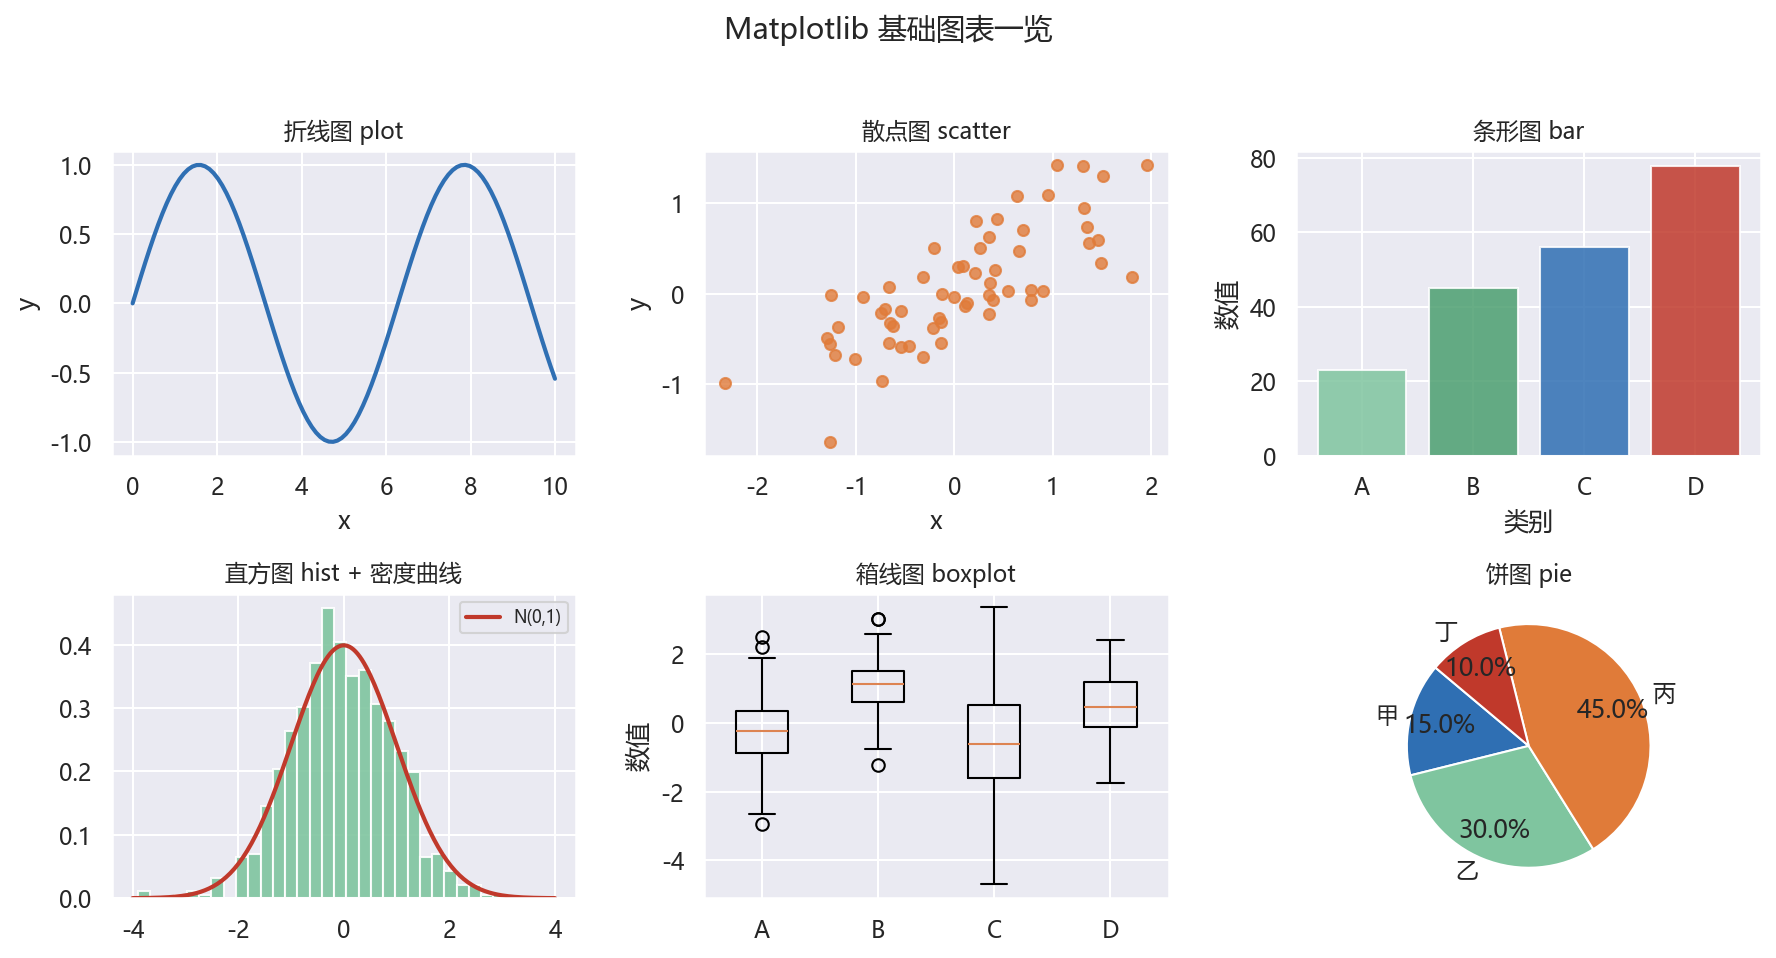
\includegraphics[keepaspectratio,alt={基础图表一览}]{figures/05-matplotlib/basic_plots.png}}
\caption{基础图表一览}
\end{figure}

\subsection{常见误区}\label{ux5e38ux89c1ux8befux533a-13}

\begin{enumerate}
\def\labelenumi{\arabic{enumi}.}
\tightlist
\item
  \textbf{只调用 \texttt{plt.plot} 不调用 \texttt{plt.show()} 或
  \texttt{savefig}}：在脚本中可能不显示也不保存，图形``消失''。
\item
  \textbf{对 \texttt{imshow} 不加
  \texttt{colorbar}}：看不出数值颜色映射。
\item
  \textbf{\texttt{plt.hist}
  直接打印可以拿到三个返回值}：\texttt{counts,\ bins,\ patches}，很多同学忽略。
\item
  \textbf{误以为 \texttt{pie} 的
  \texttt{axis(\textquotesingle{}equal\textquotesingle{})}
  可省}：不设会变成椭圆。
\item
  \textbf{随机数不设种子}：每次输出不同，课堂演示/作业请用
  \texttt{default\_rng(seed)}。
\end{enumerate}

\subsection{思考题}\label{ux601dux8003ux9898-13}

\begin{enumerate}
\def\labelenumi{\arabic{enumi}.}
\tightlist
\item
  为什么 \texttt{plt.plot(x,\ y)} 与
  \texttt{fig,\ ax\ =\ plt.subplots();\ ax.plot(x,\ y)}
  等价？它们分别管理什么状态？
\item
  \texttt{plt.scatter} 与
  \texttt{plt.plot(...,\ marker=\textquotesingle{}o\textquotesingle{})}
  对一维数据有何适用场景差异？
\item
  直方图 \texttt{density=True} 后，纵轴还能不能叫
  ``Frequency''？为什么？
\item
  3D 曲面图绘制时为什么要先 \texttt{np.meshgrid}？
\end{enumerate}

\subsection{动手练习（详见
lab）}\label{ux52a8ux624bux7ec3ux4e60ux8be6ux89c1-lab-8}

\begin{itemize}
\tightlist
\item
  绘制 \texttt{y\ =\ x\^{}3\ -\ 2x\^{}2\ +\ x} 在 \texttt{{[}-2,\ 2{]}}
  的折线图，加网格与图例；
\item
  用 \texttt{default\_rng(0)} 生成 100 个标准正态数，画 30
  箱直方图叠加理论密度曲线；
\item
  用 \texttt{tips} 数据集画 \texttt{day} 分组箱线图；
\item
  画一张 10×10 随机矩阵热力图，并对比两种 \texttt{cmap}。
\end{itemize}

\subsection{延伸阅读}\label{ux5ef6ux4f38ux9605ux8bfb-21}

\begin{itemize}
\tightlist
\item
  Matplotlib
  官方入门：https://matplotlib.org/stable/tutorials/introductory/quick\_start.html
\item
  Matplotlib
  图型画廊（Gallery）：https://matplotlib.org/stable/gallery/index.html
\item
  Seaborn 官方统计图：https://seaborn.pydata.org/tutorial.html
\end{itemize}

\section{02
图窗、布局与排版：Figure/Axes、子图、字体、坐标轴与保存}\label{ux56feux7a97ux5e03ux5c40ux4e0eux6392ux7248figureaxesux5b50ux56feux5b57ux4f53ux5750ux6807ux8f74ux4e0eux4fddux5b58}

\begin{quote}
本节对应原版 5.2 的内容，并增补学习目标、常见误区、思考题与延伸阅读。
配套图：\texttt{figures/05-matplotlib/subplots\_layout.png}（由
\texttt{build/make\_chap5\_figures.py} 生成）。
\end{quote}

\subsection{本节目标}\label{ux672cux8282ux76eeux6807-14}

\begin{itemize}
\tightlist
\item
  理解 Figure（画布）与 Axes（坐标区）的对象层级；
\item
  会用 \texttt{plt.subplots} 创建多子图并用 \texttt{ax} 逐区绘制；
\item
  会设置 \texttt{figsize/dpi}，用 \texttt{rcParams} 做全局字体与字号；
\item
  会设置轴标签、刻度、范围、网格、图例；
\item
  会使用 \texttt{tight\_layout} / \texttt{subplots\_adjust} 排版，并掌握
  \texttt{savefig} 输出。
\end{itemize}

\subsection{先修}\label{ux5148ux4fee-14}

\begin{itemize}
\tightlist
\item
  第 1 节的基础图表；NumPy 与 Pandas 基本操作。
\end{itemize}

\subsection{官方文档/参考入口}\label{ux5b98ux65b9ux6587ux6863ux53c2ux8003ux5165ux53e3-3}

\begin{itemize}
\tightlist
\item
  Matplotlib
  官方``面向对象接口''：https://matplotlib.org/stable/tutorials/introductory/usage.html\#the-object-oriented-interface
\item
  Matplotlib
  官方``文本/字体''：https://matplotlib.org/stable/users/explain/text/text\_props.html
\item
  Matplotlib
  官方``布局指南''：https://matplotlib.org/stable/tutorials/intermediate/tight\_layout\_guide.html
\end{itemize}

\begin{center}\rule{0.5\linewidth}{0.5pt}\end{center}

\subsection{2.1 Figure 与
Axes：两张``画布''}\label{figure-ux4e0e-axesux4e24ux5f20ux753bux5e03}

\begin{quote}
Matplotlib 的核心对象是 \textbf{Figure}（整张图）与
\textbf{Axes}（图中一个坐标系）。一个 Figure 可以有多个 Axes。
\end{quote}

\begin{Shaded}
\begin{Highlighting}[]
\ImportTok{import}\NormalTok{ matplotlib.pyplot }\ImportTok{as}\NormalTok{ plt}

\NormalTok{fig }\OperatorTok{=}\NormalTok{ plt.figure(figsize}\OperatorTok{=}\NormalTok{(}\DecValTok{10}\NormalTok{, }\DecValTok{4}\NormalTok{), dpi}\OperatorTok{=}\DecValTok{100}\NormalTok{)}
\NormalTok{ax }\OperatorTok{=}\NormalTok{ fig.add\_subplot(}\DecValTok{111}\NormalTok{)          }\CommentTok{\# 111 表示 1×1 网格中的第 1 个}
\BuiltInTok{print}\NormalTok{(}\StringTok{\textquotesingle{}figsize:\textquotesingle{}}\NormalTok{, fig.get\_figwidth(), }\StringTok{\textquotesingle{}x\textquotesingle{}}\NormalTok{, fig.get\_figheight())}
\BuiltInTok{print}\NormalTok{(}\StringTok{\textquotesingle{}dpi:\textquotesingle{}}\NormalTok{, fig.get\_dpi())}
\BuiltInTok{print}\NormalTok{(}\StringTok{\textquotesingle{}axes count:\textquotesingle{}}\NormalTok{, }\BuiltInTok{len}\NormalTok{(fig.axes))}
\end{Highlighting}
\end{Shaded}

\begin{Shaded}
\begin{Highlighting}[]
\NormalTok{figsize: 10.0 x 4.0}
\NormalTok{dpi: 100}
\NormalTok{axes count: 1}
\end{Highlighting}
\end{Shaded}

\begin{quote}
\texttt{plt.plot(...)} 等价于``在当前 Figure 上自动取一个 Axes
再画''，有复用代码简单、但不易同时画多子的缺点。
\end{quote}

\subsection{\texorpdfstring{2.2
子图：\texttt{plt.subplots}}{2.2 子图：plt.subplots}}\label{ux5b50ux56feplt.subplots}

\begin{Shaded}
\begin{Highlighting}[]
\ImportTok{import}\NormalTok{ matplotlib.pyplot }\ImportTok{as}\NormalTok{ plt}

\NormalTok{fig, axs }\OperatorTok{=}\NormalTok{ plt.subplots(}\DecValTok{2}\NormalTok{, }\DecValTok{2}\NormalTok{)}
\BuiltInTok{print}\NormalTok{(}\StringTok{\textquotesingle{}axs shape:\textquotesingle{}}\NormalTok{, axs.shape)}
\BuiltInTok{print}\NormalTok{(}\StringTok{\textquotesingle{}n axes:\textquotesingle{}}\NormalTok{, axs.size)}
\ControlFlowTok{for}\NormalTok{ ax }\KeywordTok{in}\NormalTok{ axs.flat:}
\NormalTok{    ax.plot([}\DecValTok{1}\NormalTok{, }\DecValTok{2}\NormalTok{], [}\DecValTok{2}\NormalTok{, }\DecValTok{1}\NormalTok{])}
\BuiltInTok{print}\NormalTok{(}\StringTok{\textquotesingle{}ok\textquotesingle{}}\NormalTok{)}
\end{Highlighting}
\end{Shaded}

\begin{Shaded}
\begin{Highlighting}[]
\NormalTok{axs shape: (2, 2)}
\NormalTok{n axes: 4}
\NormalTok{ok}
\end{Highlighting}
\end{Shaded}

\begin{quote}
\texttt{axs} 是 ndarray；用 \texttt{axs{[}0,\ 1{]}}
访问指定子区，\texttt{axs.flat} 可顺序遍历。
\end{quote}

\subsection{\texorpdfstring{2.3 图窗大小与分辨率：\texttt{figsize} 与
\texttt{dpi}}{2.3 图窗大小与分辨率：figsize 与 dpi}}\label{ux56feux7a97ux5927ux5c0fux4e0eux5206ux8fa8ux7387figsize-ux4e0e-dpi}

\begin{Shaded}
\begin{Highlighting}[]
\ImportTok{import}\NormalTok{ matplotlib.pyplot }\ImportTok{as}\NormalTok{ plt}

\NormalTok{plt.figure(figsize}\OperatorTok{=}\NormalTok{(}\DecValTok{8}\NormalTok{, }\DecValTok{6}\NormalTok{), dpi}\OperatorTok{=}\DecValTok{100}\NormalTok{)}
\NormalTok{plt.plot([}\DecValTok{1}\NormalTok{, }\DecValTok{2}\NormalTok{, }\DecValTok{3}\NormalTok{], [}\DecValTok{4}\NormalTok{, }\DecValTok{3}\NormalTok{, }\DecValTok{2}\NormalTok{])}
\CommentTok{\#\# figsize 单位英寸；dpi 为每英寸像素点数}
\BuiltInTok{print}\NormalTok{(}\StringTok{\textquotesingle{}figure created\textquotesingle{}}\NormalTok{)}
\end{Highlighting}
\end{Shaded}

输出：创建一张 8×6 英寸、100 DPI 的图窗（像素 800×600）。

\subsection{\texorpdfstring{2.4
全局字体与字号：\texttt{rcParams}}{2.4 全局字体与字号：rcParams}}\label{ux5168ux5c40ux5b57ux4f53ux4e0eux5b57ux53f7rcparams}

中文标题很常用；若不做设置，可能显示为方块。用 \texttt{rcParams}
全局设置即可：

\begin{Shaded}
\begin{Highlighting}[]
\ImportTok{import}\NormalTok{ matplotlib }\ImportTok{as}\NormalTok{ mpl}
\ImportTok{import}\NormalTok{ matplotlib.pyplot }\ImportTok{as}\NormalTok{ plt}

\NormalTok{mpl.rcParams[}\StringTok{\textquotesingle{}font.sans{-}serif\textquotesingle{}}\NormalTok{] }\OperatorTok{=}\NormalTok{ [}\StringTok{\textquotesingle{}Microsoft YaHei\textquotesingle{}}\NormalTok{, }\StringTok{\textquotesingle{}SimHei\textquotesingle{}}\NormalTok{, }\StringTok{\textquotesingle{}DejaVu Sans\textquotesingle{}}\NormalTok{]}
\NormalTok{mpl.rcParams[}\StringTok{\textquotesingle{}axes.unicode\_minus\textquotesingle{}}\NormalTok{] }\OperatorTok{=} \VariableTok{False}   \CommentTok{\# 让负号正常显示}
\NormalTok{mpl.rcParams[}\StringTok{\textquotesingle{}font.size\textquotesingle{}}\NormalTok{] }\OperatorTok{=} \DecValTok{12}
\NormalTok{plt.plot([}\DecValTok{1}\NormalTok{, }\DecValTok{2}\NormalTok{, }\DecValTok{3}\NormalTok{], [}\DecValTok{4}\NormalTok{, }\DecValTok{3}\NormalTok{, }\DecValTok{2}\NormalTok{])}
\NormalTok{plt.title(}\StringTok{\textquotesingle{}标题\textquotesingle{}}\NormalTok{)}
\BuiltInTok{print}\NormalTok{(}\StringTok{\textquotesingle{}after:\textquotesingle{}}\NormalTok{, mpl.rcParams[}\StringTok{\textquotesingle{}font.size\textquotesingle{}}\NormalTok{])}
\end{Highlighting}
\end{Shaded}

\begin{Shaded}
\begin{Highlighting}[]
\NormalTok{after: 12.0}
\end{Highlighting}
\end{Shaded}

\begin{quote}
Windows 上 \texttt{Microsoft\ YaHei} / \texttt{SimHei} 常见；Linux/macOS
可换成 \texttt{Noto\ Sans\ CJK\ SC} 或 \texttt{Arial\ Unicode\ MS}。
\end{quote}

\subsection{2.5
坐标轴：标签、范围、刻度}\label{ux5750ux6807ux8f74ux6807ux7b7eux8303ux56f4ux523bux5ea6}

\begin{Shaded}
\begin{Highlighting}[]
\ImportTok{import}\NormalTok{ matplotlib.pyplot }\ImportTok{as}\NormalTok{ plt}

\NormalTok{fig, ax }\OperatorTok{=}\NormalTok{ plt.subplots()}
\NormalTok{ax.plot([}\DecValTok{1}\NormalTok{, }\DecValTok{2}\NormalTok{, }\DecValTok{3}\NormalTok{], [}\DecValTok{4}\NormalTok{, }\DecValTok{3}\NormalTok{, }\DecValTok{2}\NormalTok{])}
\NormalTok{ax.set\_xlabel(}\StringTok{\textquotesingle{}X Axis Label\textquotesingle{}}\NormalTok{, fontsize}\OperatorTok{=}\DecValTok{14}\NormalTok{)}
\NormalTok{ax.set\_ylabel(}\StringTok{\textquotesingle{}Y Axis Label\textquotesingle{}}\NormalTok{, fontsize}\OperatorTok{=}\DecValTok{14}\NormalTok{)}
\NormalTok{ax.set\_xlim(}\DecValTok{0}\NormalTok{, }\DecValTok{4}\NormalTok{)}
\NormalTok{ax.set\_ylim(}\DecValTok{2}\NormalTok{, }\DecValTok{5}\NormalTok{)}
\NormalTok{ax.set\_xticks([}\DecValTok{1}\NormalTok{, }\DecValTok{2}\NormalTok{, }\DecValTok{3}\NormalTok{])}
\NormalTok{ax.set\_yticks([}\DecValTok{3}\NormalTok{, }\DecValTok{4}\NormalTok{])}
\BuiltInTok{print}\NormalTok{(}\StringTok{\textquotesingle{}xlim:\textquotesingle{}}\NormalTok{, }\BuiltInTok{tuple}\NormalTok{(}\BuiltInTok{float}\NormalTok{(v) }\ControlFlowTok{for}\NormalTok{ v }\KeywordTok{in}\NormalTok{ ax.get\_xlim()))}
\BuiltInTok{print}\NormalTok{(}\StringTok{\textquotesingle{}ylim:\textquotesingle{}}\NormalTok{, }\BuiltInTok{tuple}\NormalTok{(}\BuiltInTok{float}\NormalTok{(v) }\ControlFlowTok{for}\NormalTok{ v }\KeywordTok{in}\NormalTok{ ax.get\_ylim()))}
\BuiltInTok{print}\NormalTok{(}\StringTok{\textquotesingle{}xticks:\textquotesingle{}}\NormalTok{, [}\BuiltInTok{int}\NormalTok{(v) }\ControlFlowTok{for}\NormalTok{ v }\KeywordTok{in}\NormalTok{ ax.get\_xticks()])}
\end{Highlighting}
\end{Shaded}

\begin{Shaded}
\begin{Highlighting}[]
\NormalTok{xlim: (0.0, 4.0)}
\NormalTok{ylim: (2.0, 5.0)}
\NormalTok{xticks: [1, 2, 3]}
\end{Highlighting}
\end{Shaded}

\subsection{2.6 网格与图例}\label{ux7f51ux683cux4e0eux56feux4f8b}

\begin{Shaded}
\begin{Highlighting}[]
\ImportTok{import}\NormalTok{ matplotlib.pyplot }\ImportTok{as}\NormalTok{ plt}

\NormalTok{fig, ax }\OperatorTok{=}\NormalTok{ plt.subplots()}
\NormalTok{ax.plot([}\DecValTok{1}\NormalTok{, }\DecValTok{2}\NormalTok{, }\DecValTok{3}\NormalTok{], [}\DecValTok{4}\NormalTok{, }\DecValTok{3}\NormalTok{, }\DecValTok{2}\NormalTok{], label}\OperatorTok{=}\StringTok{\textquotesingle{}line 1\textquotesingle{}}\NormalTok{)}
\NormalTok{ax.plot([}\DecValTok{1}\NormalTok{, }\DecValTok{2}\NormalTok{, }\DecValTok{3}\NormalTok{], [}\DecValTok{2}\NormalTok{, }\DecValTok{3}\NormalTok{, }\DecValTok{4}\NormalTok{], label}\OperatorTok{=}\StringTok{\textquotesingle{}line 2\textquotesingle{}}\NormalTok{)}
\NormalTok{ax.grid(color}\OperatorTok{=}\StringTok{\textquotesingle{}gray\textquotesingle{}}\NormalTok{, linestyle}\OperatorTok{=}\StringTok{\textquotesingle{}{-}{-}\textquotesingle{}}\NormalTok{, linewidth}\OperatorTok{=}\FloatTok{0.5}\NormalTok{)}
\NormalTok{ax.legend()}
\BuiltInTok{print}\NormalTok{(}\StringTok{\textquotesingle{}handles:\textquotesingle{}}\NormalTok{, }\BuiltInTok{len}\NormalTok{(ax.get\_legend().get\_texts()))}
\end{Highlighting}
\end{Shaded}

\begin{Shaded}
\begin{Highlighting}[]
\NormalTok{handles: 2}
\end{Highlighting}
\end{Shaded}

\begin{quote}
图例 \texttt{loc} 可选
\texttt{\textquotesingle{}best\textquotesingle{}}、\texttt{\textquotesingle{}upper\ right\textquotesingle{}}、\texttt{\textquotesingle{}lower\ left\textquotesingle{}}
等；\texttt{grid} 可设颜色/线型/线宽。
\end{quote}

\subsection{\texorpdfstring{2.7 排版：\texttt{tight\_layout} 与
\texttt{subplots\_adjust}}{2.7 排版：tight\_layout 与 subplots\_adjust}}\label{ux6392ux7248tight_layout-ux4e0e-subplots_adjust}

\texttt{tight\_layout} 自动让子图不重叠；\texttt{subplots\_adjust}
手动控制边界与间距。

\begin{Shaded}
\begin{Highlighting}[]
\ImportTok{import}\NormalTok{ matplotlib.pyplot }\ImportTok{as}\NormalTok{ plt}

\NormalTok{fig, axs }\OperatorTok{=}\NormalTok{ plt.subplots(}\DecValTok{2}\NormalTok{, }\DecValTok{2}\NormalTok{, figsize}\OperatorTok{=}\NormalTok{(}\DecValTok{9}\NormalTok{, }\DecValTok{6}\NormalTok{))}
\ControlFlowTok{for}\NormalTok{ ax }\KeywordTok{in}\NormalTok{ axs.flat:}
\NormalTok{    ax.plot([}\DecValTok{1}\NormalTok{, }\DecValTok{2}\NormalTok{, }\DecValTok{3}\NormalTok{], [}\DecValTok{2}\NormalTok{, }\DecValTok{1}\NormalTok{, }\DecValTok{3}\NormalTok{])}
\NormalTok{fig.suptitle(}\StringTok{\textquotesingle{}示例\textquotesingle{}}\NormalTok{, fontsize}\OperatorTok{=}\DecValTok{14}\NormalTok{)}
\NormalTok{fig.tight\_layout()                    }\CommentTok{\# 自动排版，推荐}
\CommentTok{\#\# fig.subplots\_adjust(left=0.1, right=0.9, top=0.9, bottom=0.1, wspace=0.3, hspace=0.3)}
\BuiltInTok{print}\NormalTok{(}\StringTok{\textquotesingle{}layout ok\textquotesingle{}}\NormalTok{)}
\end{Highlighting}
\end{Shaded}

输出：\texttt{layout\ ok}，运行后得到整洁的 2×2 子图（见下方示例图）。

\begin{figure}
\centering
\pandocbounded{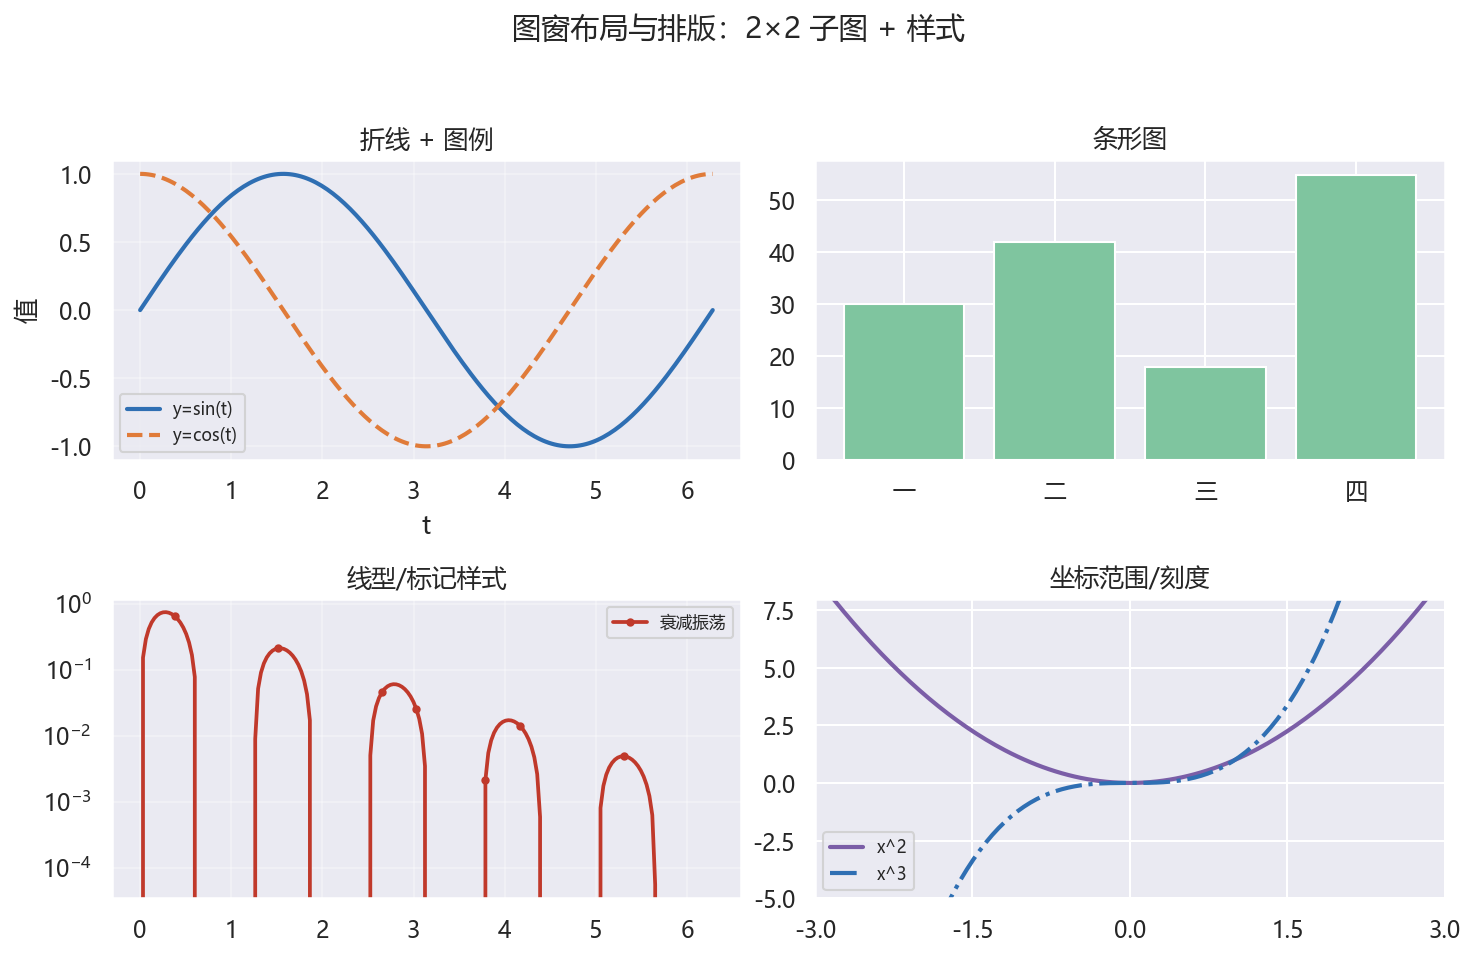
\includegraphics[keepaspectratio,alt={图窗布局示例}]{figures/05-matplotlib/subplots_layout.png}}
\caption{图窗布局示例}
\end{figure}

\subsection{\texorpdfstring{2.8
保存图像：\texttt{savefig}}{2.8 保存图像：savefig}}\label{ux4fddux5b58ux56feux50cfsavefig}

\begin{Shaded}
\begin{Highlighting}[]
\ImportTok{import}\NormalTok{ matplotlib.pyplot }\ImportTok{as}\NormalTok{ plt}
\ImportTok{import}\NormalTok{ os}

\NormalTok{plt.figure(figsize}\OperatorTok{=}\NormalTok{(}\DecValTok{8}\NormalTok{, }\DecValTok{6}\NormalTok{), dpi}\OperatorTok{=}\DecValTok{100}\NormalTok{)}
\NormalTok{plt.plot([}\DecValTok{1}\NormalTok{, }\DecValTok{2}\NormalTok{, }\DecValTok{3}\NormalTok{], [}\DecValTok{4}\NormalTok{, }\DecValTok{3}\NormalTok{, }\DecValTok{2}\NormalTok{])}
\NormalTok{plt.savefig(}\StringTok{\textquotesingle{}my\_plot.png\textquotesingle{}}\NormalTok{, dpi}\OperatorTok{=}\DecValTok{150}\NormalTok{)}
\BuiltInTok{print}\NormalTok{(}\StringTok{\textquotesingle{}exists:\textquotesingle{}}\NormalTok{, os.path.exists(}\StringTok{\textquotesingle{}my\_plot.png\textquotesingle{}}\NormalTok{))}
\end{Highlighting}
\end{Shaded}

\begin{Shaded}
\begin{Highlighting}[]
\NormalTok{exists: True}
\end{Highlighting}
\end{Shaded}

\begin{quote}
\texttt{savefig} 的 \texttt{dpi} 可单独覆盖图窗
DPI；格式由扩展名决定（\texttt{png} / \texttt{jpg} / \texttt{pdf} /
\texttt{svg} 等）。
\end{quote}

\subsection{常见误区}\label{ux5e38ux89c1ux8befux533a-14}

\begin{enumerate}
\def\labelenumi{\arabic{enumi}.}
\tightlist
\item
  \textbf{混用 \texttt{plt} 与 \texttt{ax} 接口}：在面向对象代码中继续用
  \texttt{plt.title}
  可能作用于``当前''轴，子图多了易错。建议一个图中要么纯函数式、要么纯面向对象。
\item
  \textbf{忘记 \texttt{tight\_layout}}：子图标题、轴标签互相重叠。
\item
  \textbf{\texttt{set\_xticks} 与 \texttt{set\_xticklabels}
  混用}：前者设刻度位置，后者改刻度文字。
\item
  \textbf{把 \texttt{figsize} 单位当像素}：实际单位是英寸，配合
  \texttt{dpi} 才得到像素。
\item
  \textbf{\texttt{rcParams} 在 \texttt{seaborn.set\_theme}
  之后设置}：否则字体被覆盖回 Arial（见第 3 节）。
\end{enumerate}

\subsection{思考题}\label{ux601dux8003ux9898-14}

\begin{enumerate}
\def\labelenumi{\arabic{enumi}.}
\tightlist
\item
  \texttt{fig,\ axs\ =\ plt.subplots(3,\ 4)} 中 \texttt{axs.shape}
  是多少？如何访问第 2 行第 3 列子图？
\item
  为什么 \texttt{plt.show()}
  不能在无窗口服务器上显示图形？此时用哪种方法输出？
\item
  \texttt{tight\_layout} 和 \texttt{subplots\_adjust}
  的区别是什么？各自适合什么场景？
\item
  要在每个子图上画不同内容并共用同一 \texttt{x} 轴，\texttt{axs.flat}
  与显式下标哪种更清晰？
\end{enumerate}

\subsection{动手练习（详见
lab）}\label{ux52a8ux624bux7ec3ux4e60ux8be6ux89c1-lab-9}

\begin{itemize}
\tightlist
\item
  创建 2×3 子图，分别画 sin、cos、tan、exp、log、x\^{}2；
\item
  用 \texttt{rcParams} 设置全局字号 12，并为每个子图加中文标题；
\item
  上一题做完后调用 \texttt{fig.tight\_layout()} 观察差异；
\item
  用 \texttt{savefig} 导出 300 DPI 的 PDF。
\end{itemize}

\subsection{延伸阅读}\label{ux5ef6ux4f38ux9605ux8bfb-22}

\begin{itemize}
\tightlist
\item
  Matplotlib 官方``Pyplot
  教程''：https://matplotlib.org/stable/tutorials/pyplot.html
\item
  Matplotlib 官方``面向对象
  API''：https://matplotlib.org/stable/tutorials/introductory/usage.html\#the-object-oriented-interface
\item
  Matplotlib
  官方``文本/字体''：https://matplotlib.org/stable/users/explain/text/text\_props.html
\end{itemize}

\section{03 Seaborn
美化：主题、统计图与分面}\label{seaborn-ux7f8eux5316ux4e3bux9898ux7edfux8ba1ux56feux4e0eux5206ux9762}

\begin{quote}
本节对应原版 5.3 的内容，并增补学习目标、常见误区、思考题与延伸阅读。
配套图：\texttt{figures/05-matplotlib/seaborn\_style.png}（由
\texttt{build/make\_chap5\_figures.py} 生成）。
\end{quote}

\subsection{本节目标}\label{ux672cux8282ux76eeux6807-15}

\begin{itemize}
\tightlist
\item
  理解 Seaborn 与 Matplotlib 的关系；
\item
  会用 \texttt{set\_theme} / \texttt{set\_style} 切换全局主题；
\item
  会用
  \texttt{histplot}、\texttt{kdeplot}、\texttt{boxplot}、\texttt{violinplot}、\texttt{heatmap}
  做统计可视化；
\item
  会用 \texttt{FacetGrid} / \texttt{pairplot} 做分面与成对图；
\item
  会与 Matplotlib 的 \texttt{subplots} 结合做多子图报告图。
\end{itemize}

\subsection{先修}\label{ux5148ux4fee-15}

\begin{itemize}
\tightlist
\item
  第 1--2 节的内容；Pandas DataFrame（\texttt{load\_dataset} 返回的就是
  DataFrame）。
\end{itemize}

\subsection{官方文档/参考入口}\label{ux5b98ux65b9ux6587ux6863ux53c2ux8003ux5165ux53e3-4}

\begin{itemize}
\tightlist
\item
  Seaborn 官方教程：https://seaborn.pydata.org/tutorial.html
\item
  Seaborn 官方 API：https://seaborn.pydata.org/api.html
\item
  Matplotlib
  官方图型画廊：https://matplotlib.org/stable/gallery/index.html
\end{itemize}

\begin{center}\rule{0.5\linewidth}{0.5pt}\end{center}

\subsection{3.1 Seaborn 是什么}\label{seaborn-ux662fux4ec0ux4e48}

Seaborn 建立在 Matplotlib 之上，提供：更口语化的函数名、可直接接受
DataFrame 列名、内置统计（如 KDE、分组箱线）、以及一套美观默认主题。

\textbf{注意}：\texttt{sns.set\_theme(style="darkgrid")} 会重置
Matplotlib 的
\texttt{rcParams}（包括字体），所以\textbf{设置主题后要重新设中文字体}，否则中文标题会变方块。

\begin{Shaded}
\begin{Highlighting}[]
\ImportTok{import}\NormalTok{ seaborn }\ImportTok{as}\NormalTok{ sns}
\ImportTok{import}\NormalTok{ matplotlib }\ImportTok{as}\NormalTok{ mpl}
\ImportTok{import}\NormalTok{ matplotlib.pyplot }\ImportTok{as}\NormalTok{ plt}

\NormalTok{sns.set\_theme(style}\OperatorTok{=}\StringTok{"darkgrid"}\NormalTok{)}
\NormalTok{mpl.rcParams[}\StringTok{"font.sans{-}serif"}\NormalTok{] }\OperatorTok{=}\NormalTok{ [}\StringTok{"Microsoft YaHei"}\NormalTok{, }\StringTok{"SimHei"}\NormalTok{, }\StringTok{"DejaVu Sans"}\NormalTok{]}
\NormalTok{mpl.rcParams[}\StringTok{"axes.unicode\_minus"}\NormalTok{] }\OperatorTok{=} \VariableTok{False}

\NormalTok{tips }\OperatorTok{=}\NormalTok{ sns.load\_dataset(}\StringTok{"tips"}\NormalTok{)}
\BuiltInTok{print}\NormalTok{(}\StringTok{"tips shape:"}\NormalTok{, tips.shape)}
\BuiltInTok{print}\NormalTok{(tips.head(}\DecValTok{3}\NormalTok{).to\_string(index}\OperatorTok{=}\VariableTok{False}\NormalTok{))}
\end{Highlighting}
\end{Shaded}

\begin{Shaded}
\begin{Highlighting}[]
\NormalTok{tips shape: (244, 7)}
\NormalTok{ total\_bill  tip    sex smoker day   time  size}
\NormalTok{      16.99 1.01 Female     No Sun Dinner     2}
\NormalTok{      10.34 1.66   Male     No Sun Dinner     3}
\NormalTok{      21.01 3.50   Male     No Sun Dinner     3}
\end{Highlighting}
\end{Shaded}

\begin{quote}
常见主题：\texttt{darkgrid}（默认）、\texttt{whitegrid}、\texttt{dark}、\texttt{white}、\texttt{ticks}。
\end{quote}

\subsection{3.2 在子图中使用
Seaborn}\label{ux5728ux5b50ux56feux4e2dux4f7fux7528-seaborn}

\begin{Shaded}
\begin{Highlighting}[]
\ImportTok{import}\NormalTok{ seaborn }\ImportTok{as}\NormalTok{ sns}
\ImportTok{import}\NormalTok{ matplotlib.pyplot }\ImportTok{as}\NormalTok{ plt}

\NormalTok{tips }\OperatorTok{=}\NormalTok{ sns.load\_dataset(}\StringTok{"tips"}\NormalTok{)}
\NormalTok{fig, axes }\OperatorTok{=}\NormalTok{ plt.subplots(}\DecValTok{2}\NormalTok{, }\DecValTok{2}\NormalTok{, figsize}\OperatorTok{=}\NormalTok{(}\DecValTok{10}\NormalTok{, }\DecValTok{8}\NormalTok{))}
\NormalTok{sns.lineplot(x}\OperatorTok{=}\StringTok{"tip"}\NormalTok{, y}\OperatorTok{=}\StringTok{"total\_bill"}\NormalTok{, data}\OperatorTok{=}\NormalTok{tips, ax}\OperatorTok{=}\NormalTok{axes[}\DecValTok{0}\NormalTok{, }\DecValTok{0}\NormalTok{])}
\NormalTok{sns.barplot(x}\OperatorTok{=}\StringTok{"sex"}\NormalTok{, y}\OperatorTok{=}\StringTok{"total\_bill"}\NormalTok{, data}\OperatorTok{=}\NormalTok{tips, ax}\OperatorTok{=}\NormalTok{axes[}\DecValTok{0}\NormalTok{, }\DecValTok{1}\NormalTok{])}
\NormalTok{sns.scatterplot(x}\OperatorTok{=}\StringTok{"total\_bill"}\NormalTok{, y}\OperatorTok{=}\StringTok{"tip"}\NormalTok{, hue}\OperatorTok{=}\StringTok{"sex"}\NormalTok{, data}\OperatorTok{=}\NormalTok{tips, ax}\OperatorTok{=}\NormalTok{axes[}\DecValTok{1}\NormalTok{, }\DecValTok{0}\NormalTok{])}
\NormalTok{sns.histplot(data}\OperatorTok{=}\NormalTok{tips[}\StringTok{"total\_bill"}\NormalTok{], ax}\OperatorTok{=}\NormalTok{axes[}\DecValTok{1}\NormalTok{, }\DecValTok{1}\NormalTok{])}
\NormalTok{plt.tight\_layout()}
\BuiltInTok{print}\NormalTok{(}\StringTok{"subplots ok:"}\NormalTok{, axes.shape)}
\end{Highlighting}
\end{Shaded}

\begin{Shaded}
\begin{Highlighting}[]
\NormalTok{subplots ok: (2, 2)}
\end{Highlighting}
\end{Shaded}

\begin{quote}
把 \texttt{data=} 传入 DataFrame，并给
\texttt{x}/\texttt{y}/\texttt{hue} 传列名，Seaborn 自动分组。
\end{quote}

\subsection{3.3 常用统计图}\label{ux5e38ux7528ux7edfux8ba1ux56fe}

\subsubsection{3.3.1 频率直方图 +
核密度线}\label{ux9891ux7387ux76f4ux65b9ux56fe-ux6838ux5bc6ux5ea6ux7ebf}

\begin{Shaded}
\begin{Highlighting}[]
\ImportTok{import}\NormalTok{ seaborn }\ImportTok{as}\NormalTok{ sns}
\ImportTok{import}\NormalTok{ matplotlib.pyplot }\ImportTok{as}\NormalTok{ plt}

\NormalTok{tips }\OperatorTok{=}\NormalTok{ sns.load\_dataset(}\StringTok{"tips"}\NormalTok{)}
\NormalTok{sns.histplot(tips, x}\OperatorTok{=}\StringTok{"total\_bill"}\NormalTok{, kde}\OperatorTok{=}\VariableTok{True}\NormalTok{)}
\NormalTok{plt.show()}
\end{Highlighting}
\end{Shaded}

\subsubsection{3.3.2
概率密度曲线}\label{ux6982ux7387ux5bc6ux5ea6ux66f2ux7ebf}

\begin{Shaded}
\begin{Highlighting}[]
\NormalTok{sns.kdeplot(tips[}\StringTok{"total\_bill"}\NormalTok{], fill}\OperatorTok{=}\VariableTok{True}\NormalTok{)}
\NormalTok{plt.show()}
\end{Highlighting}
\end{Shaded}

\begin{quote}
新版 seaborn 用 \texttt{fill=True}（旧版 \texttt{shade=True} 已弃用）。
\end{quote}

\subsubsection{3.3.3
箱线图与提琴图}\label{ux7bb1ux7ebfux56feux4e0eux63d0ux7434ux56fe}

\begin{Shaded}
\begin{Highlighting}[]
\ImportTok{import}\NormalTok{ seaborn }\ImportTok{as}\NormalTok{ sns}
\ImportTok{import}\NormalTok{ matplotlib.pyplot }\ImportTok{as}\NormalTok{ plt}

\NormalTok{tips }\OperatorTok{=}\NormalTok{ sns.load\_dataset(}\StringTok{"tips"}\NormalTok{)}
\NormalTok{fig, axes }\OperatorTok{=}\NormalTok{ plt.subplots(}\DecValTok{1}\NormalTok{, }\DecValTok{2}\NormalTok{, figsize}\OperatorTok{=}\NormalTok{(}\DecValTok{9}\NormalTok{, }\FloatTok{3.5}\NormalTok{))}
\NormalTok{sns.boxplot(x}\OperatorTok{=}\StringTok{"day"}\NormalTok{, y}\OperatorTok{=}\StringTok{"total\_bill"}\NormalTok{, data}\OperatorTok{=}\NormalTok{tips, ax}\OperatorTok{=}\NormalTok{axes[}\DecValTok{0}\NormalTok{])}
\NormalTok{sns.violinplot(x}\OperatorTok{=}\StringTok{"day"}\NormalTok{, y}\OperatorTok{=}\StringTok{"total\_bill"}\NormalTok{, data}\OperatorTok{=}\NormalTok{tips, ax}\OperatorTok{=}\NormalTok{axes[}\DecValTok{1}\NormalTok{])}
\BuiltInTok{print}\NormalTok{(}\StringTok{"boxes:"}\NormalTok{, }\BuiltInTok{len}\NormalTok{(axes[}\DecValTok{0}\NormalTok{].containers), }\StringTok{"violins:"}\NormalTok{, }\BuiltInTok{len}\NormalTok{(axes[}\DecValTok{1}\NormalTok{].collections))}
\end{Highlighting}
\end{Shaded}

\begin{Shaded}
\begin{Highlighting}[]
\NormalTok{boxes: 1  violins: 4}
\end{Highlighting}
\end{Shaded}

\subsubsection{3.3.4 热力图}\label{ux70edux529bux56fe}

\begin{Shaded}
\begin{Highlighting}[]
\ImportTok{import}\NormalTok{ seaborn }\ImportTok{as}\NormalTok{ sns}
\ImportTok{import}\NormalTok{ matplotlib.pyplot }\ImportTok{as}\NormalTok{ plt}

\NormalTok{flights }\OperatorTok{=}\NormalTok{ sns.load\_dataset(}\StringTok{"flights"}\NormalTok{)}
\NormalTok{flights\_pivot }\OperatorTok{=}\NormalTok{ flights.pivot\_table(index}\OperatorTok{=}\StringTok{"month"}\NormalTok{, columns}\OperatorTok{=}\StringTok{"year"}\NormalTok{, values}\OperatorTok{=}\StringTok{"passengers"}\NormalTok{, observed}\OperatorTok{=}\VariableTok{False}\NormalTok{)}
\NormalTok{sns.heatmap(flights\_pivot, annot}\OperatorTok{=}\VariableTok{True}\NormalTok{, fmt}\OperatorTok{=}\StringTok{".0f"}\NormalTok{)}
\BuiltInTok{print}\NormalTok{(}\StringTok{"pivot shape:"}\NormalTok{, flights\_pivot.shape)}
\end{Highlighting}
\end{Shaded}

\begin{Shaded}
\begin{Highlighting}[]
\NormalTok{pivot shape: (12, 12)}
\end{Highlighting}
\end{Shaded}

\subsubsection{3.3.5 成对关系图}\label{ux6210ux5bf9ux5173ux7cfbux56fe}

\begin{Shaded}
\begin{Highlighting}[]
\ImportTok{import}\NormalTok{ seaborn }\ImportTok{as}\NormalTok{ sns}

\NormalTok{tips }\OperatorTok{=}\NormalTok{ sns.load\_dataset(}\StringTok{"tips"}\NormalTok{)}
\NormalTok{g }\OperatorTok{=}\NormalTok{ sns.pairplot(tips, hue}\OperatorTok{=}\StringTok{"day"}\NormalTok{)}
\BuiltInTok{print}\NormalTok{(}\StringTok{"pairplot grid shape:"}\NormalTok{, g.axes.shape)}
\end{Highlighting}
\end{Shaded}

\begin{Shaded}
\begin{Highlighting}[]
\NormalTok{pairplot grid shape: (3, 3)}
\end{Highlighting}
\end{Shaded}

\subsection{\texorpdfstring{3.4 分面与多图：\texttt{FacetGrid} /
\texttt{PairGrid}}{3.4 分面与多图：FacetGrid / PairGrid}}\label{ux5206ux9762ux4e0eux591aux56fefacetgrid-pairgrid}

\begin{Shaded}
\begin{Highlighting}[]
\ImportTok{import}\NormalTok{ seaborn }\ImportTok{as}\NormalTok{ sns}
\ImportTok{import}\NormalTok{ matplotlib.pyplot }\ImportTok{as}\NormalTok{ plt}

\NormalTok{tips }\OperatorTok{=}\NormalTok{ sns.load\_dataset(}\StringTok{"tips"}\NormalTok{)}
\NormalTok{g }\OperatorTok{=}\NormalTok{ sns.FacetGrid(tips, col}\OperatorTok{=}\StringTok{"day"}\NormalTok{, col\_wrap}\OperatorTok{=}\DecValTok{4}\NormalTok{)}
\NormalTok{g.}\BuiltInTok{map}\NormalTok{(sns.lineplot, }\StringTok{"total\_bill"}\NormalTok{, }\StringTok{"tip"}\NormalTok{)}
\NormalTok{g.add\_legend()}
\BuiltInTok{print}\NormalTok{(}\StringTok{"FacetGrid axes:"}\NormalTok{, }\BuiltInTok{len}\NormalTok{(g.axes.flat))}
\end{Highlighting}
\end{Shaded}

\begin{Shaded}
\begin{Highlighting}[]
\NormalTok{FacetGrid axes: 4}
\end{Highlighting}
\end{Shaded}

\begin{quote}
\texttt{FacetGrid} 按列取值把数据切成多个子图；\texttt{col\_wrap}
控制每行放几个。\texttt{PairGrid} 则用于变量两两成对。
\end{quote}

\begin{figure}
\centering
\pandocbounded{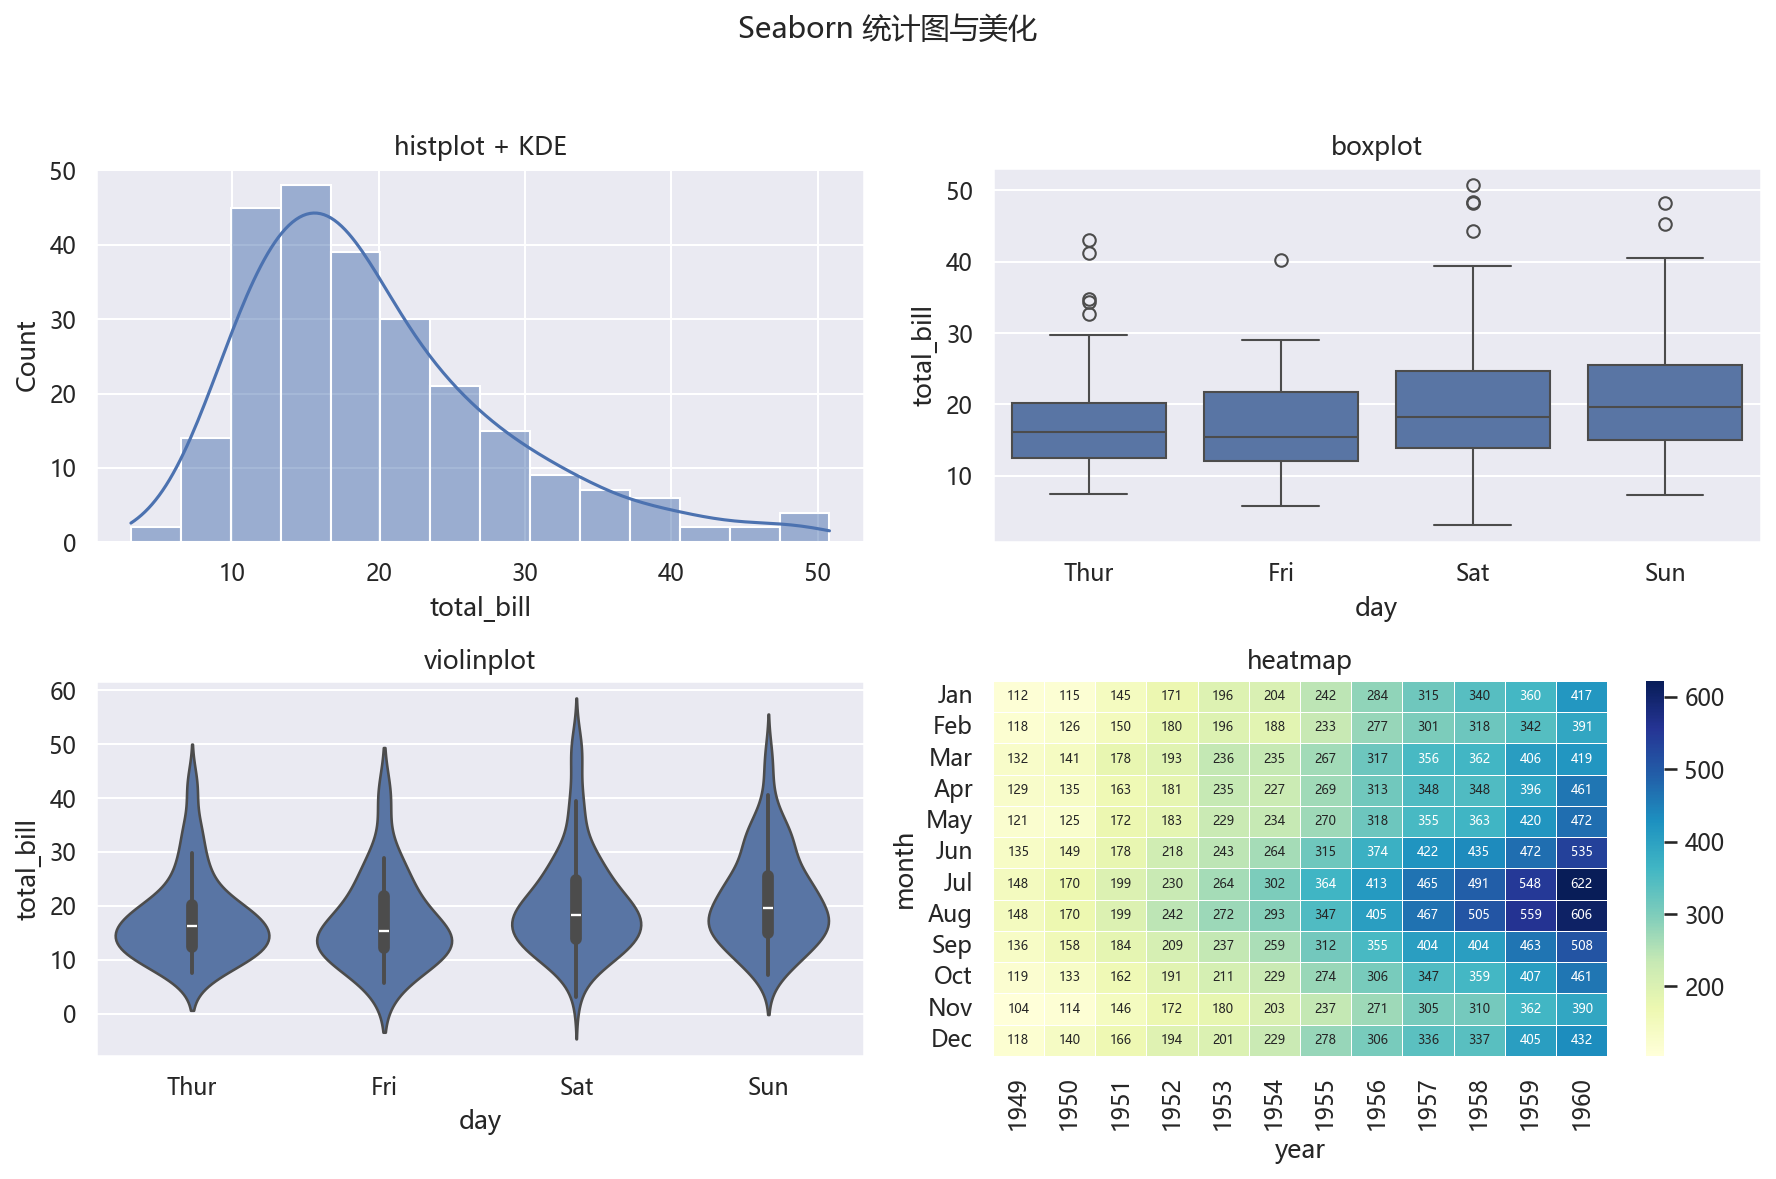
\includegraphics[keepaspectratio,alt={Seaborn 统计图与美化}]{figures/05-matplotlib/seaborn_style.png}}
\caption{Seaborn 统计图与美化}
\end{figure}

\subsection{常见误区}\label{ux5e38ux89c1ux8befux533a-15}

\begin{enumerate}
\def\labelenumi{\arabic{enumi}.}
\tightlist
\item
  \textbf{\texttt{set\_theme} 之后不重设中文字体}：中文标题变方块。
\item
  \textbf{把旧版 \texttt{shade=True} 当新 API}：新版本改为
  \texttt{fill=True}，旧参数已弃用。
\item
  \textbf{\texttt{sns.boxplot} 返回的 \texttt{ax} 与 Matplotlib 子图混用
  \texttt{plt.title}}：多个子图时易错。
\item
  \textbf{\texttt{load\_dataset} 依赖网络}：若要离线教学，可先用
  \texttt{pd.DataFrame(...)} 构造样例数据。
\item
  \textbf{给 \texttt{heatmap} 的 \texttt{fmt="d"} 传浮点数据}：应改用
  \texttt{fmt=".0f"} 或 \texttt{.2f}。
\end{enumerate}

\subsection{思考题}\label{ux601dux8003ux9898-15}

\begin{enumerate}
\def\labelenumi{\arabic{enumi}.}
\tightlist
\item
  \texttt{sns.set\_theme} 与 \texttt{plt.style.use} 有何异同？
\item
  \texttt{boxplot} 与 \texttt{violinplot} 分别适合什么场景？
\item
  为什么 \texttt{FacetGrid} 比手动 \texttt{subplots}
  循环更适合``按类别分面''？
\item
  在 Seaborn 图中能否继续用 Matplotlib 的
  \texttt{set\_xticks}？如何操作？
\end{enumerate}

\subsection{动手练习（详见
lab）}\label{ux52a8ux624bux7ec3ux4e60ux8be6ux89c1-lab-10}

\begin{itemize}
\tightlist
\item
  用 \texttt{tips} 画 \texttt{day} 分组的箱线图，并切换
  \texttt{whitegrid} / \texttt{ticks} 主题对比；
\item
  用 \texttt{flights} 透视表画热力图，并自定义 \texttt{cmap}；
\item
  用 \texttt{penguins} 数据集做一对 \texttt{pairplot}；
\item
  用 \texttt{FacetGrid} 按 \texttt{sex} 分面画 \texttt{total\_bill}
  的直方图。
\end{itemize}

\subsection{延伸阅读}\label{ux5ef6ux4f38ux9605ux8bfb-23}

\begin{itemize}
\tightlist
\item
  Seaborn 官方教程：https://seaborn.pydata.org/tutorial.html
\item
  Seaborn 官方 API：https://seaborn.pydata.org/api.html
\item
  Matplotlib + Seaborn
  结合示例：https://seaborn.pydata.org/examples/index.html
\end{itemize}

\section{04
综合案例：传感器信号分析与分组报告图}\label{ux7efcux5408ux6848ux4f8bux4f20ux611fux5668ux4fe1ux53f7ux5206ux6790ux4e0eux5206ux7ec4ux62a5ux544aux56fe}

\begin{quote}
本章新增综合案例，用于把 01--03 的知识串起来：\textbf{基础图表 +
多子图/排版 + Seaborn 统计图}。 所有代码均可在 matplotlib ≥ 3.8、seaborn
≥ 0.13 环境运行；配图由 \texttt{build/make\_chap5\_figures.py} 生成。
\end{quote}

\subsection{案例背景}\label{ux6848ux4f8bux80ccux666f-2}

假设你拿到一段``传感器信号''采样（含噪声）与一批分组测量值，需要输出一张\textbf{数据分析报告图}：

\begin{enumerate}
\def\labelenumi{\arabic{enumi}.}
\tightlist
\item
  左上：时间序列折线图，把原始信号与滑动平均后的平滑信号叠在一起；
\item
  右上：信号幅值直方图 + 核密度估计（Seaborn）；
\item
  左下：对照组 / 实验组的分组散点图；
\item
  右下：几个变量之间的相关矩阵热力图。
\end{enumerate}

这正是第 1 章的``数据能画出来'' + 第 2 章的``多子图排版'' + 第 3
章``Seaborn 统计图''的联合应用。

\subsection{步骤
1：生成合成信号并平滑}\label{ux6b65ux9aa4-1ux751fux6210ux5408ux6210ux4fe1ux53f7ux5e76ux5e73ux6ed1}

\begin{Shaded}
\begin{Highlighting}[]
\ImportTok{import}\NormalTok{ numpy }\ImportTok{as}\NormalTok{ np}
\ImportTok{import}\NormalTok{ pandas }\ImportTok{as}\NormalTok{ pd}
\ImportTok{import}\NormalTok{ matplotlib.pyplot }\ImportTok{as}\NormalTok{ plt}
\ImportTok{import}\NormalTok{ seaborn }\ImportTok{as}\NormalTok{ sns}

\NormalTok{rng }\OperatorTok{=}\NormalTok{ np.random.default\_rng(}\DecValTok{2025}\NormalTok{)   }\CommentTok{\# 固定种子，保证可复现}
\NormalTok{n }\OperatorTok{=} \DecValTok{400}
\NormalTok{t }\OperatorTok{=}\NormalTok{ np.linspace(}\DecValTok{0}\NormalTok{, }\DecValTok{20}\NormalTok{, n)}
\NormalTok{signal }\OperatorTok{=} \DecValTok{3} \OperatorTok{*}\NormalTok{ np.sin(}\DecValTok{2} \OperatorTok{*}\NormalTok{ np.pi }\OperatorTok{*} \FloatTok{0.25} \OperatorTok{*}\NormalTok{ t) }\OperatorTok{+} \FloatTok{0.6} \OperatorTok{*}\NormalTok{ np.cos(}\DecValTok{2} \OperatorTok{*}\NormalTok{ np.pi }\OperatorTok{*} \FloatTok{1.1} \OperatorTok{*}\NormalTok{ t) }\OperatorTok{+} \FloatTok{0.8}
\NormalTok{y }\OperatorTok{=}\NormalTok{ signal }\OperatorTok{+}\NormalTok{ rng.normal(}\DecValTok{0}\NormalTok{, }\FloatTok{0.5}\NormalTok{, n)}
\NormalTok{smoothed }\OperatorTok{=}\NormalTok{ pd.Series(y).rolling(window}\OperatorTok{=}\DecValTok{15}\NormalTok{, center}\OperatorTok{=}\VariableTok{True}\NormalTok{).mean().to\_numpy()}

\BuiltInTok{print}\NormalTok{(}\StringTok{"信号长度 n ="}\NormalTok{, n)}
\BuiltInTok{print}\NormalTok{(}\StringTok{"原始信号  均值 ="}\NormalTok{, }\BuiltInTok{round}\NormalTok{(}\BuiltInTok{float}\NormalTok{(y.mean()), }\DecValTok{3}\NormalTok{), }\StringTok{" 标准差 ="}\NormalTok{, }\BuiltInTok{round}\NormalTok{(}\BuiltInTok{float}\NormalTok{(y.std()), }\DecValTok{3}\NormalTok{))}
\BuiltInTok{print}\NormalTok{(}\StringTok{"平滑信号  均值 ="}\NormalTok{, }\BuiltInTok{round}\NormalTok{(}\BuiltInTok{float}\NormalTok{(np.nanmean(smoothed)), }\DecValTok{3}\NormalTok{))}
\BuiltInTok{print}\NormalTok{(}\StringTok{"平滑信号 前 5 个 ="}\NormalTok{, np.}\BuiltInTok{round}\NormalTok{(smoothed[:}\DecValTok{5}\NormalTok{], }\DecValTok{3}\NormalTok{))}
\end{Highlighting}
\end{Shaded}

\begin{Shaded}
\begin{Highlighting}[]
\NormalTok{信号长度 n = 400}
\NormalTok{原始信号  均值 = 0.795  标准差 = 2.244}
\NormalTok{平滑信号  均值 = 0.797}
\NormalTok{平滑信号 前 5 个 = [nan nan nan nan nan]}
\end{Highlighting}
\end{Shaded}

\begin{quote}
\texttt{rolling(window=15,\ center=True)}
做中心化滑动平均；两端窗口不满时为 NaN，属正常现象。
\end{quote}

\subsection{步骤
2：生成分组数据与相关矩阵}\label{ux6b65ux9aa4-2ux751fux6210ux5206ux7ec4ux6570ux636eux4e0eux76f8ux5173ux77e9ux9635}

\begin{Shaded}
\begin{Highlighting}[]
\NormalTok{rng2 }\OperatorTok{=}\NormalTok{ np.random.default\_rng(}\DecValTok{1}\NormalTok{)}
\NormalTok{group }\OperatorTok{=}\NormalTok{ rng2.choice([}\StringTok{"对照组"}\NormalTok{, }\StringTok{"实验组"}\NormalTok{], size}\OperatorTok{=}\DecValTok{250}\NormalTok{, p}\OperatorTok{=}\NormalTok{[}\FloatTok{0.5}\NormalTok{, }\FloatTok{0.5}\NormalTok{])}
\NormalTok{val }\OperatorTok{=}\NormalTok{ np.where(group }\OperatorTok{==} \StringTok{"实验组"}\NormalTok{, rng2.normal(}\FloatTok{5.2}\NormalTok{, }\FloatTok{1.1}\NormalTok{, }\DecValTok{250}\NormalTok{), rng2.normal(}\FloatTok{4.0}\NormalTok{, }\FloatTok{1.0}\NormalTok{, }\DecValTok{250}\NormalTok{))}

\NormalTok{df\_corr }\OperatorTok{=}\NormalTok{ pd.DataFrame(\{}
    \StringTok{"x1"}\NormalTok{: rng2.normal(}\DecValTok{0}\NormalTok{, }\DecValTok{1}\NormalTok{, }\DecValTok{300}\NormalTok{),}
    \StringTok{"x2"}\NormalTok{: rng2.normal(}\DecValTok{0}\NormalTok{, }\DecValTok{1}\NormalTok{, }\DecValTok{300}\NormalTok{),}
    \StringTok{"x3"}\NormalTok{: rng2.normal(}\DecValTok{0}\NormalTok{, }\DecValTok{1}\NormalTok{, }\DecValTok{300}\NormalTok{),}
\NormalTok{\})}
\NormalTok{df\_corr[}\StringTok{"x4"}\NormalTok{] }\OperatorTok{=} \FloatTok{0.8} \OperatorTok{*}\NormalTok{ df\_corr[}\StringTok{"x1"}\NormalTok{] }\OperatorTok{+}\NormalTok{ rng2.normal(}\DecValTok{0}\NormalTok{, }\FloatTok{0.6}\NormalTok{, }\DecValTok{300}\NormalTok{)}
\NormalTok{corr }\OperatorTok{=}\NormalTok{ df\_corr.corr()}

\BuiltInTok{print}\NormalTok{(}\StringTok{"对照组均值 ="}\NormalTok{, }\BuiltInTok{round}\NormalTok{(}\BuiltInTok{float}\NormalTok{(val[group }\OperatorTok{==} \StringTok{"对照组"}\NormalTok{].mean()), }\DecValTok{3}\NormalTok{))}
\BuiltInTok{print}\NormalTok{(}\StringTok{"实验组均值 ="}\NormalTok{, }\BuiltInTok{round}\NormalTok{(}\BuiltInTok{float}\NormalTok{(val[group }\OperatorTok{==} \StringTok{"实验组"}\NormalTok{].mean()), }\DecValTok{3}\NormalTok{))}
\BuiltInTok{print}\NormalTok{(}\StringTok{"相关系数 x1{-}x4 ="}\NormalTok{, }\BuiltInTok{round}\NormalTok{(}\BuiltInTok{float}\NormalTok{(corr.loc[}\StringTok{"x1"}\NormalTok{, }\StringTok{"x4"}\NormalTok{]), }\DecValTok{3}\NormalTok{))}
\BuiltInTok{print}\NormalTok{(}\StringTok{"相关系数 x1{-}x2 ="}\NormalTok{, }\BuiltInTok{round}\NormalTok{(}\BuiltInTok{float}\NormalTok{(corr.loc[}\StringTok{"x1"}\NormalTok{, }\StringTok{"x2"}\NormalTok{]), }\DecValTok{3}\NormalTok{))}
\BuiltInTok{print}\NormalTok{()}
\BuiltInTok{print}\NormalTok{(corr.}\BuiltInTok{round}\NormalTok{(}\DecValTok{2}\NormalTok{).to\_string())}
\end{Highlighting}
\end{Shaded}

\begin{Shaded}
\begin{Highlighting}[]
\NormalTok{对照组均值 = 3.874}
\NormalTok{实验组均值 = 5.274}
\NormalTok{相关系数 x1{-}x4 = 0.819}
\NormalTok{相关系数 x1{-}x2 = {-}0.097}

\NormalTok{      x1    x2    x3    x4}
\NormalTok{x1  1.00 {-}0.10  0.06  0.82}
\NormalTok{x2 {-}0.10  1.00 {-}0.05 {-}0.07}
\NormalTok{x3  0.06 {-}0.05  1.00  0.07}
\NormalTok{x4  0.82 {-}0.07  0.07  1.00}
\end{Highlighting}
\end{Shaded}

\begin{quote}
因为构造时 \texttt{x4} 由 \texttt{x1} 主导，所以 \texttt{x1–x4}
相关系数约 0.8，热力图一眼可辨。
\end{quote}

\subsection{步骤 3：绘制 2×2
报告图}\label{ux6b65ux9aa4-3ux7ed8ux5236-22-ux62a5ux544aux56fe}

\begin{quote}
本步依赖步骤 1/2 中定义的
\texttt{t}、\texttt{y}、\texttt{smoothed}、\texttt{group}、\texttt{val}、\texttt{corr}，请按顺序运行。
\end{quote}

\begin{Shaded}
\begin{Highlighting}[]
\CommentTok{\#\# 中文字体（注意：set\_theme 会覆盖，这里放在绘图前重新设置）}
\ImportTok{import}\NormalTok{ matplotlib }\ImportTok{as}\NormalTok{ mpl}
\NormalTok{mpl.rcParams[}\StringTok{"font.sans{-}serif"}\NormalTok{] }\OperatorTok{=}\NormalTok{ [}\StringTok{"Microsoft YaHei"}\NormalTok{, }\StringTok{"SimHei"}\NormalTok{, }\StringTok{"DejaVu Sans"}\NormalTok{]}
\NormalTok{mpl.rcParams[}\StringTok{"axes.unicode\_minus"}\NormalTok{] }\OperatorTok{=} \VariableTok{False}

\NormalTok{fig, axes }\OperatorTok{=}\NormalTok{ plt.subplots(}\DecValTok{2}\NormalTok{, }\DecValTok{2}\NormalTok{, figsize}\OperatorTok{=}\NormalTok{(}\DecValTok{12}\NormalTok{, }\FloatTok{8.5}\NormalTok{))}
\NormalTok{fig.suptitle(}\StringTok{"综合案例：传感器信号观测与分组分析"}\NormalTok{, fontsize}\OperatorTok{=}\DecValTok{15}\NormalTok{)}

\NormalTok{axes[}\DecValTok{0}\NormalTok{, }\DecValTok{0}\NormalTok{].plot(t, y, color}\OperatorTok{=}\StringTok{"\#c8d8e8"}\NormalTok{, lw}\OperatorTok{=}\DecValTok{1}\NormalTok{, label}\OperatorTok{=}\StringTok{"原始信号"}\NormalTok{)}
\NormalTok{axes[}\DecValTok{0}\NormalTok{, }\DecValTok{0}\NormalTok{].plot(t, smoothed, color}\OperatorTok{=}\StringTok{"\#c0392b"}\NormalTok{, lw}\OperatorTok{=}\FloatTok{2.2}\NormalTok{, label}\OperatorTok{=}\StringTok{"滑动平均(窗口=15)"}\NormalTok{)}
\NormalTok{axes[}\DecValTok{0}\NormalTok{, }\DecValTok{0}\NormalTok{].set\_title(}\StringTok{"时间序列：原始信号 vs 平滑"}\NormalTok{)}
\NormalTok{axes[}\DecValTok{0}\NormalTok{, }\DecValTok{0}\NormalTok{].set\_xlabel(}\StringTok{"时间 t"}\NormalTok{)}\OperatorTok{;}\NormalTok{ axes[}\DecValTok{0}\NormalTok{, }\DecValTok{0}\NormalTok{].set\_ylabel(}\StringTok{"幅值"}\NormalTok{)}
\NormalTok{axes[}\DecValTok{0}\NormalTok{, }\DecValTok{0}\NormalTok{].legend(fontsize}\OperatorTok{=}\DecValTok{8}\NormalTok{)}\OperatorTok{;}\NormalTok{ axes[}\DecValTok{0}\NormalTok{, }\DecValTok{0}\NormalTok{].grid(alpha}\OperatorTok{=}\FloatTok{0.3}\NormalTok{)}

\NormalTok{sns.histplot(x}\OperatorTok{=}\NormalTok{y, kde}\OperatorTok{=}\VariableTok{True}\NormalTok{, color}\OperatorTok{=}\StringTok{"\#2f6fb3"}\NormalTok{, ax}\OperatorTok{=}\NormalTok{axes[}\DecValTok{0}\NormalTok{, }\DecValTok{1}\NormalTok{])}
\NormalTok{axes[}\DecValTok{0}\NormalTok{, }\DecValTok{1}\NormalTok{].set\_title(}\StringTok{"信号幅值分布"}\NormalTok{)}
\NormalTok{axes[}\DecValTok{0}\NormalTok{, }\DecValTok{1}\NormalTok{].set\_xlabel(}\StringTok{"幅值"}\NormalTok{)}

\NormalTok{axes[}\DecValTok{1}\NormalTok{, }\DecValTok{0}\NormalTok{].scatter(group[group }\OperatorTok{==} \StringTok{"对照组"}\NormalTok{], val[group }\OperatorTok{==} \StringTok{"对照组"}\NormalTok{],}
\NormalTok{                   color}\OperatorTok{=}\StringTok{"\#7fc59f"}\NormalTok{, s}\OperatorTok{=}\DecValTok{22}\NormalTok{, alpha}\OperatorTok{=}\FloatTok{0.75}\NormalTok{, label}\OperatorTok{=}\StringTok{"对照组"}\NormalTok{)}
\NormalTok{axes[}\DecValTok{1}\NormalTok{, }\DecValTok{0}\NormalTok{].scatter(group[group }\OperatorTok{==} \StringTok{"实验组"}\NormalTok{], val[group }\OperatorTok{==} \StringTok{"实验组"}\NormalTok{],}
\NormalTok{                   color}\OperatorTok{=}\StringTok{"\#e07b39"}\NormalTok{, s}\OperatorTok{=}\DecValTok{22}\NormalTok{, alpha}\OperatorTok{=}\FloatTok{0.75}\NormalTok{, label}\OperatorTok{=}\StringTok{"实验组"}\NormalTok{)}
\NormalTok{axes[}\DecValTok{1}\NormalTok{, }\DecValTok{0}\NormalTok{].set\_title(}\StringTok{"分组散点图"}\NormalTok{)}
\NormalTok{axes[}\DecValTok{1}\NormalTok{, }\DecValTok{0}\NormalTok{].set\_xlabel(}\StringTok{"分组"}\NormalTok{)}\OperatorTok{;}\NormalTok{ axes[}\DecValTok{1}\NormalTok{, }\DecValTok{0}\NormalTok{].set\_ylabel(}\StringTok{"测量值"}\NormalTok{)}
\NormalTok{axes[}\DecValTok{1}\NormalTok{, }\DecValTok{0}\NormalTok{].legend(fontsize}\OperatorTok{=}\DecValTok{8}\NormalTok{)}\OperatorTok{;}\NormalTok{ axes[}\DecValTok{1}\NormalTok{, }\DecValTok{0}\NormalTok{].grid(alpha}\OperatorTok{=}\FloatTok{0.3}\NormalTok{)}

\NormalTok{sns.heatmap(corr, annot}\OperatorTok{=}\VariableTok{True}\NormalTok{, fmt}\OperatorTok{=}\StringTok{".2f"}\NormalTok{, cmap}\OperatorTok{=}\StringTok{"coolwarm"}\NormalTok{, vmin}\OperatorTok{={-}}\DecValTok{1}\NormalTok{, vmax}\OperatorTok{=}\DecValTok{1}\NormalTok{,}
\NormalTok{            ax}\OperatorTok{=}\NormalTok{axes[}\DecValTok{1}\NormalTok{, }\DecValTok{1}\NormalTok{], annot\_kws}\OperatorTok{=}\NormalTok{\{}\StringTok{"fontsize"}\NormalTok{: }\DecValTok{9}\NormalTok{\})}
\NormalTok{axes[}\DecValTok{1}\NormalTok{, }\DecValTok{1}\NormalTok{].set\_title(}\StringTok{"变量间相关矩阵热力图"}\NormalTok{)}

\NormalTok{fig.tight\_layout(rect}\OperatorTok{=}\NormalTok{[}\DecValTok{0}\NormalTok{, }\DecValTok{0}\NormalTok{, }\DecValTok{1}\NormalTok{, }\FloatTok{0.95}\NormalTok{])}
\NormalTok{fig.savefig(}\StringTok{"case\_study.png"}\NormalTok{, dpi}\OperatorTok{=}\DecValTok{150}\NormalTok{)}
\BuiltInTok{print}\NormalTok{(}\StringTok{"已保存 case\_study.png"}\NormalTok{)}
\end{Highlighting}
\end{Shaded}

输出：\texttt{已保存\ case\_study.png}，并得到下图。

\begin{figure}
\centering
\pandocbounded{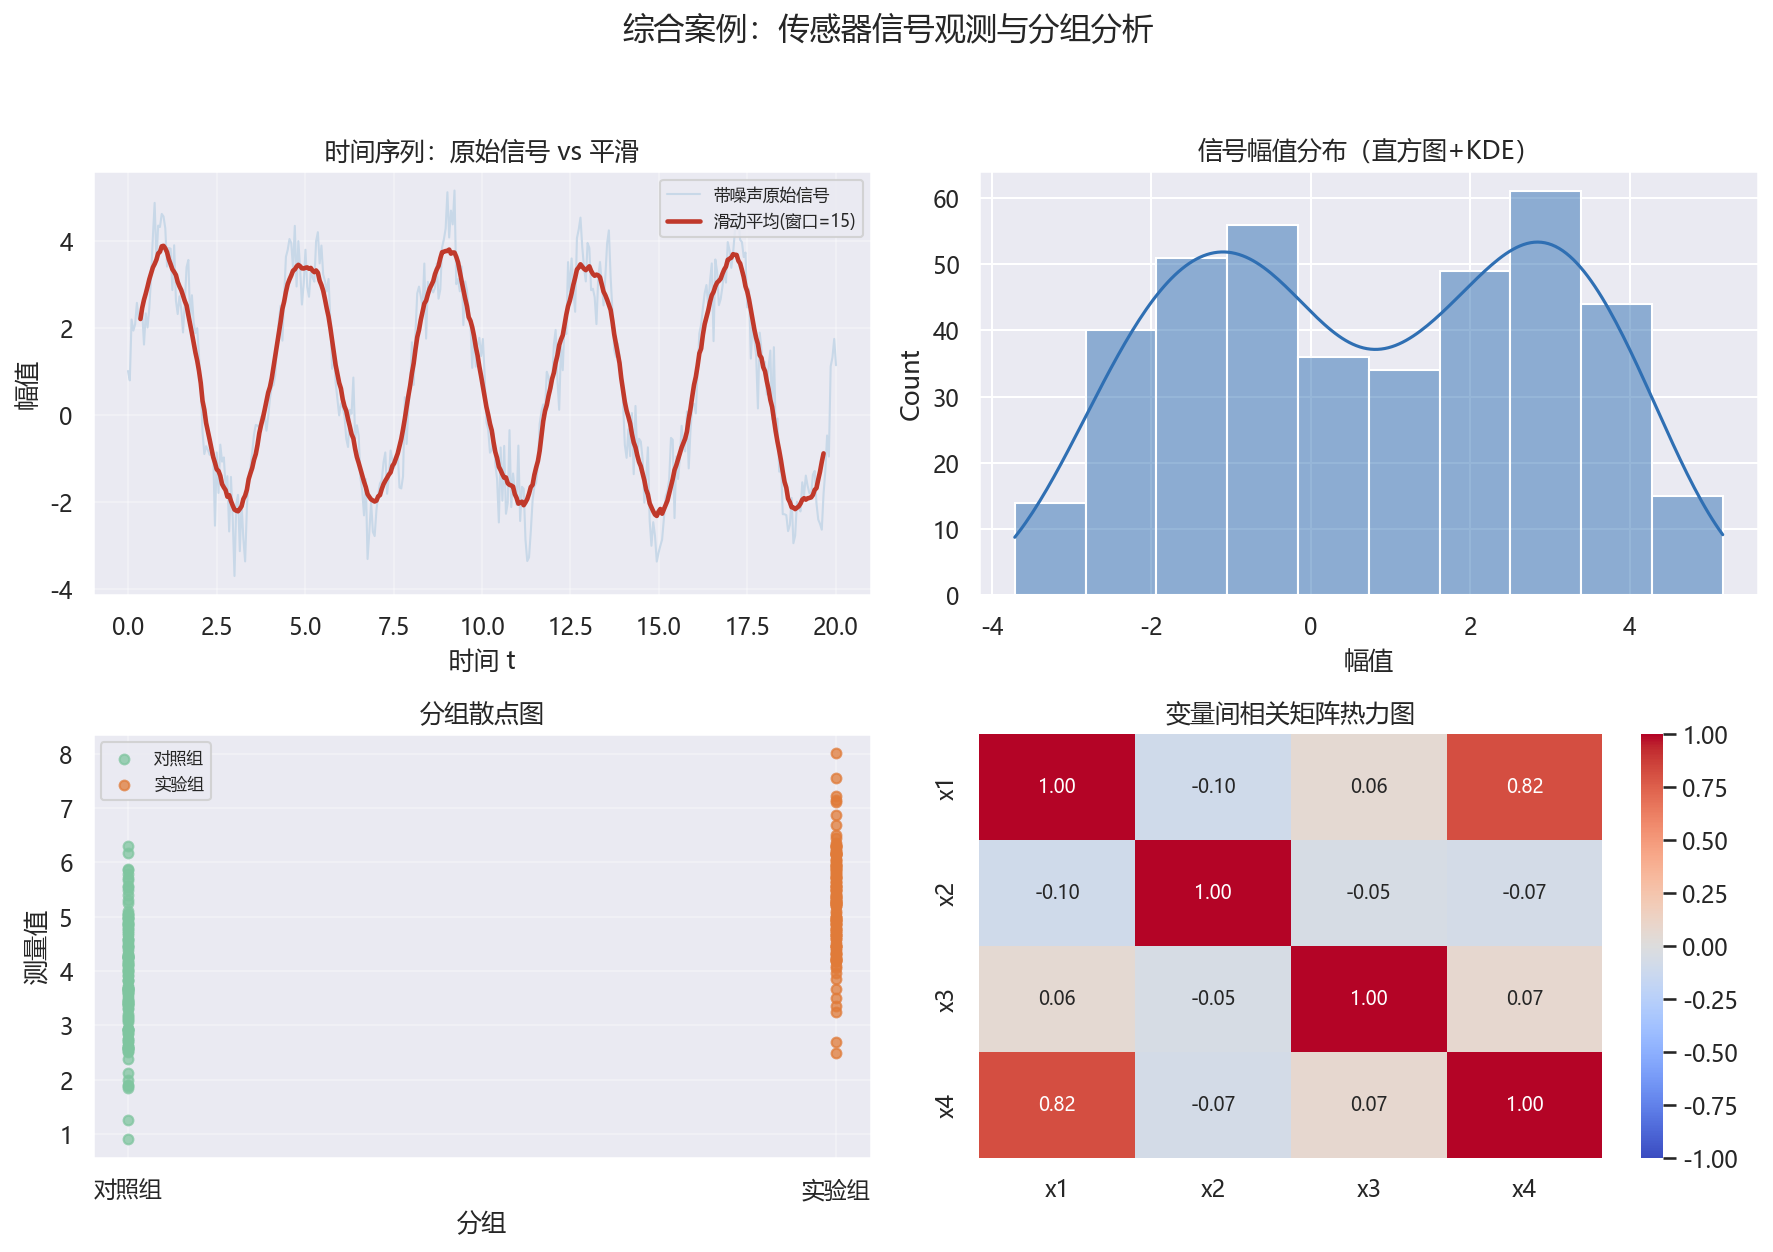
\includegraphics[keepaspectratio,alt={综合案例报告图}]{figures/05-matplotlib/case_study.png}}
\caption{综合案例报告图}
\end{figure}

\subsection{分析与延伸}\label{ux5206ux6790ux4e0eux5ef6ux4f38}

\begin{itemize}
\tightlist
\item
  \textbf{左上}：原始信号噪声明显，滑动平均后波形更平滑------直观体会``平滑窗口''对信噪比的影响；
\item
  \textbf{右上}：信号幅值近似正态分布（叠加噪声的多频正弦叠加），KDE
  与直方图吻合；
\item
  \textbf{左下}：实验组测量值整体高于对照组，散点图可直接看出两组的中心差异；
\item
  \textbf{右下}：\texttt{x1} 与 \texttt{x4} 相关系数约
  0.8，热力图让``共线性''一目了然。
\end{itemize}

\subsubsection{拓展任务}\label{ux62d3ux5c55ux4efbux52a1-7}

\begin{enumerate}
\def\labelenumi{\arabic{enumi}.}
\tightlist
\item
  把平滑窗口从 15 改为 5 / 31，比较左上图平滑程度与失真；
\item
  用 \texttt{sns.kdeplot} 分开画对照/实验两组的密度曲线，观察重叠区域；
\item
  把相关矩阵改用 \texttt{sns.clustermap} 展示变量聚类；
\item
  将报告图导出为 PDF，并比较不同 \texttt{dpi} 的文件大小。
\end{enumerate}

\subsection{延伸阅读}\label{ux5ef6ux4f38ux9605ux8bfb-24}

\begin{itemize}
\tightlist
\item
  Matplotlib
  多子图：https://matplotlib.org/stable/tutorials/intermediate/subplots.html
\item
  Seaborn
  分布图：https://seaborn.pydata.org/generated/seaborn.histplot.html
\item
  Pandas
  \texttt{rolling}：https://pandas.pydata.org/docs/reference/api/pandas.DataFrame.rolling.html
\end{itemize}

\section{05
常见误区与技巧}\label{ux5e38ux89c1ux8befux533aux4e0eux6280ux5de7-4}

\begin{quote}
本章为新增``查漏补缺''页：把学生最容易踩的坑集中列出，并给出正确的写法和性能技巧。
\end{quote}

\subsection{1.
高频误区速查表}\label{ux9ad8ux9891ux8befux533aux901fux67e5ux8868-4}

{\def\LTcaptype{none} % do not increment counter
\begin{longtable}[]{@{}
  >{\raggedright\arraybackslash}p{(\linewidth - 6\tabcolsep) * \real{0.2500}}
  >{\raggedright\arraybackslash}p{(\linewidth - 6\tabcolsep) * \real{0.2500}}
  >{\raggedright\arraybackslash}p{(\linewidth - 6\tabcolsep) * \real{0.2500}}
  >{\raggedright\arraybackslash}p{(\linewidth - 6\tabcolsep) * \real{0.2500}}@{}}
\toprule\noalign{}
\begin{minipage}[b]{\linewidth}\raggedright
\#
\end{minipage} & \begin{minipage}[b]{\linewidth}\raggedright
误区 / 错误写法
\end{minipage} & \begin{minipage}[b]{\linewidth}\raggedright
正确做法
\end{minipage} & \begin{minipage}[b]{\linewidth}\raggedright
原因
\end{minipage} \\
\midrule\noalign{}
\endhead
\bottomrule\noalign{}
\endlastfoot
1 & 只 \texttt{plt.plot} 不 \texttt{plt.show()}/\texttt{savefig} &
脚本中用 \texttt{plt.savefig}；交互环境用 \texttt{plt.show()} &
图可能``画了不显示/不保存'' \\
2 & 面向对象代码里混用 \texttt{plt.title} & 用
\texttt{ax.set\_title(...)} & 多子图时 \texttt{plt}
作用于当前轴，易错 \\
3 & 忘记 \texttt{ax.set\_xticks} 与 \texttt{set\_xticklabels} 的区别 &
前者设位置，后者改文字 & 两个函数语义不同 \\
4 & 误以为 \texttt{figsize} 是像素 & 单位是英寸，需乘 \texttt{dpi}
得到像素 & 单位语义错误 \\
5 & \texttt{rcParams} 在 seaborn \texttt{set\_theme} 之前设置 &
主题之后重新设置字体 & \texttt{set\_theme} 会重置
\texttt{font.sans-serif} \\
6 & 对 \texttt{heatmap} 传 \texttt{fmt="d"} 而数据是浮点 & 改用
\texttt{fmt=".0f"} 或 \texttt{.2f} & 格式码与数据类型不匹配 \\
7 & 用旧版 \texttt{shade=True} & 用 \texttt{fill=True} &
新版参数已改名 \\
8 & \texttt{plt.subplots(2,2)} 后用 \texttt{plt.subplot()} 再画 &
统一用返回的 \texttt{axs.flat} & 两个接口混用会叠加到错误的轴 \\
9 & 忘记 \texttt{np.meshgrid} 就画 3D 曲面 & 先 \texttt{np.meshgrid}
生成 2D 网格 & 曲面需要网格化的 X, Y, Z \\
10 & 误以为一张图只能有一个 Figure & 一个脚本可多 Figure；用
\texttt{plt.figure()} 新建 & 状态管理理解偏差 \\
11 & 中文标题变方块还不设字体 & 设
\texttt{rcParams{[}"font.sans-serif"{]}\ =\ {[}"Microsoft\ YaHei",\ ...{]}}
& 默认字体不含中文字形 \\
12 & 频繁 \texttt{plt.show()} 后又想改 \texttt{rcParams} &
先设全局参数再绘图 & \texttt{rcParams} 影响后续创建的对象 \\
\end{longtable}
}

\subsection{2. 原理级难点：面向对象 vs
函数式}\label{ux539fux7406ux7ea7ux96beux70b9ux9762ux5411ux5bf9ux8c61-vs-ux51fdux6570ux5f0f}

\begin{Shaded}
\begin{Highlighting}[]
\CommentTok{\#\# 函数式：简单，但一张图只有一个“当前轴”}
\ImportTok{import}\NormalTok{ matplotlib.pyplot }\ImportTok{as}\NormalTok{ plt}
\NormalTok{plt.plot([}\DecValTok{1}\NormalTok{, }\DecValTok{2}\NormalTok{, }\DecValTok{3}\NormalTok{], [}\DecValTok{1}\NormalTok{, }\DecValTok{4}\NormalTok{, }\DecValTok{9}\NormalTok{])}
\NormalTok{plt.title(}\StringTok{"one"}\NormalTok{)}

\CommentTok{\#\# 面向对象：显式管理多个轴}
\NormalTok{fig, axs }\OperatorTok{=}\NormalTok{ plt.subplots(}\DecValTok{2}\NormalTok{, }\DecValTok{2}\NormalTok{)}
\NormalTok{axs[}\DecValTok{0}\NormalTok{, }\DecValTok{0}\NormalTok{].plot([}\DecValTok{1}\NormalTok{, }\DecValTok{2}\NormalTok{], [}\DecValTok{2}\NormalTok{, }\DecValTok{1}\NormalTok{])}
\NormalTok{axs[}\DecValTok{0}\NormalTok{, }\DecValTok{0}\NormalTok{].set\_title(}\StringTok{"topleft"}\NormalTok{)}
\NormalTok{axs[}\DecValTok{1}\NormalTok{, }\DecValTok{1}\NormalTok{].scatter([}\DecValTok{1}\NormalTok{, }\DecValTok{2}\NormalTok{], [}\DecValTok{3}\NormalTok{, }\DecValTok{4}\NormalTok{])}
\end{Highlighting}
\end{Shaded}

\begin{quote}
经验：\textbf{单图且临时探索用函数式；多子图/出版图用面向对象}。二者混用是学生最常见的返工原因。
\end{quote}

\subsection{3.
性能与排版技巧}\label{ux6027ux80fdux4e0eux6392ux7248ux6280ux5de7}

\begin{itemize}
\tightlist
\item
  \textbf{优先 \texttt{tight\_layout()}}：比反复
  \texttt{subplots\_adjust} 手工试更快；
\item
  \textbf{用 \texttt{ax.set\_xticks}/\texttt{set\_xticklabels}
  控制刻度}：避免默认 0,0.5,1 与数据不匹配；
\item
  \textbf{大量子图用 \texttt{mosaic} /
  \texttt{GridSpec}}：\texttt{fig,\ axs\ =\ plt.subplots}
  只支持均匀网格；不均匀用 \texttt{GridSpec} 更灵活；
\item
  \textbf{图片给 \texttt{dpi}}：论文图建议 300 DPI，屏幕演示 100--150
  DPI；
\item
  \textbf{复用同一 \texttt{fig} 与 \texttt{ax}}：一个循环里不断
  \texttt{plt.figure()} 会开几十个窗口，消耗内存；
\item
  \textbf{\texttt{savefig} 前先
  \texttt{fig.tight\_layout()}}，否则标题会被裁剪。
\end{itemize}

\subsection{4. 调试建议}\label{ux8c03ux8bd5ux5efaux8bae-4}

\begin{enumerate}
\def\labelenumi{\arabic{enumi}.}
\tightlist
\item
  中文变方块：先检查 \texttt{mpl.rcParams{[}"font.sans-serif"{]}}
  是否在用中文字体，再看 \texttt{axes.unicode\_minus}；
\item
  图形为空/只显示一张：确认是否用了 \texttt{plt.figure()} 后又
  \texttt{plt.subplot} 建了新轴；
\item
  子图重叠：调用 \texttt{fig.tight\_layout()}；
\item
  坐标范围不对：打印 \texttt{ax.get\_xlim()} / \texttt{ax.get\_ylim()}
  调试；
\item
  图例不出现：检查 \texttt{plot(label=...)} 是否每一条都有
  \texttt{label}，再看 \texttt{legend()}；
\item
  保存的文件打不开：确认有写权限，扩展名正确，且 \texttt{savefig} 前没有
  \texttt{close}。
\end{enumerate}

\subsection{5.
本章小结（自测）}\label{ux672cux7ae0ux5c0fux7ed3ux81eaux6d4b-2}

\begin{itemize}
\tightlist
\item[$\square$]
  能说出 Figure 与 Axes 的关系；
\item[$\square$]
  能创建 2×2 子图并在指定位置画图；
\item[$\square$]
  能用 \texttt{rcParams} 让中文正常显示；
\item[$\square$]
  能设置颜色/线宽/线型/标记/图例/网格；
\item[$\square$]
  能用 \texttt{savefig} 输出 300 DPI 图片；
\item[$\square$]
  能用 Seaborn 画 \texttt{histplot} / \texttt{boxplot} /
  \texttt{heatmap} / \texttt{FacetGrid}；
\item[$\square$]
  能独立完成 04 综合案例的报告图。
\end{itemize}

\subsection{延伸阅读}\label{ux5ef6ux4f38ux9605ux8bfb-25}

\begin{itemize}
\tightlist
\item
  Matplotlib 官方 FAQ：https://matplotlib.org/stable/faq/index.html
\item
  Matplotlib
  官方``Cheatsheets''：https://matplotlib.org/stable/cheatsheets/index.html
\item
  Seaborn 官方``Choosing color
  palettes''：https://seaborn.pydata.org/tutorial/color\_palettes.html
\end{itemize}

\newpage
